\documentclass{article}[12pt]
\usepackage{physics}
\usepackage{setspace}
\usepackage{amsmath}
\usepackage{mathrsfs}
\usepackage{amssymb}
\usepackage{feynmp-auto}
\usepackage{tgtermes}
\usepackage{graphicx}
\usepackage{booktabs}
\usepackage{array}
\usepackage{caption}
\usepackage{listings}
\usepackage{xcolor}
\usepackage{helvet}
\usepackage{float}
\definecolor{codegreen}{rgb}{0,0.6,0}
\definecolor{codegray}{rgb}{0.5,0.5,0.5}
\definecolor{codepurple}{rgb}{0.58,0,0.82}
\definecolor{backcolour}{rgb}{0.95,0.95,0.92}
\definecolor{lightgray}{rgb}{0.95,0.95,0.95}
\bibliography{Master_Thesis}
\lstdefinestyle{mystyle}{
    backgroundcolor=\color{lightgray},   
    commentstyle=\color{codegreen},
    keywordstyle=\color{magenta},
    numberstyle=\tiny\color{codegray},
    stringstyle=\color{codepurple},
    basicstyle=\fontfamily{pcr}\selectfont\footnotesize,
    breakatwhitespace=false,         
    breaklines=true,                 
    captionpos=b,                    
    keepspaces=true,                 
    numbers=left,                    
    numbersep=5pt,                  
    showspaces=false,                
    showstringspaces=false,
    showtabs=false,                  
    tabsize=2
}
\numberwithin{equation}{section}
\lstset{style=mystyle}
\captionsetup{font=footnotesize}
\newcommand{\RN}[1]{%s
  \textup{\uppercase\expandafter{\romannumeral#1}}%
}
\usepackage{geometry}
\geometry{
 a4paper,
 left=25.4mm,
 right=25.4mm,
 top=30mm,
 bottom=25.4mm
 }
\begin{document}
\section{Introduction}
\begin{spacing}{1.5}

The study of the correlation between the particle-like systems in a many-body framework can predict a wide range of novel phenomena in condensed matter physics, especially in the aspects of phase transition. 
This perspective is crucial for the recent advances in quantum technologies such as quantum simulators implemented through optical lattice, superconducting circuits, and quantum materials (e.g., quantum dots).

The Phase transition between metal and insulator is defined as a rapid transition of conductivity. In the metallic phase, inside the material structure, there are free electrons exist and make available to electric current flows throughout the material, in the insulating phase the electrons are bonded tightly with atoms which hinders the flow of electric current.Several theories have been developed to describe this phase transition phenomenon. In the Mott transition, the change of conductivity is explained through the Coulomb interactions between the electrons. While the density of the electrons inside the material becomes saturated, the interaction effect leads to repulsion between the particles which impedes current flow. Alternatively, In Andersen's transition model, the transition between the two phases is explained from more microscopic points of view by using the concept of disorder and impurities.

\pagebreak
\subsection{Summary}
In our study, we investigate the phase transition of a resistively shunted Josephson junction within the framework of the quantum impurity model. 
We establish a quantum mechanical framework based on the state vector of the macroscopic Josephson junction model. 
As starting in the very first step, we use impurity solving method (Non-crossing approximation, One-crossing approximation, TOA) in thermally stable state with Matsubara formalism , then evaluate the evolution of correlation of energy change ratio.

By employing the framework of strong correlation method, we expect a concrete description of the phase transition in a resistively shunted Josephson junction which is an ongoing debate. The precise nature of this transition is to be addressed through the analysis of the quantum state of electrons.
\begin{figure}[htbp]
  \centerline{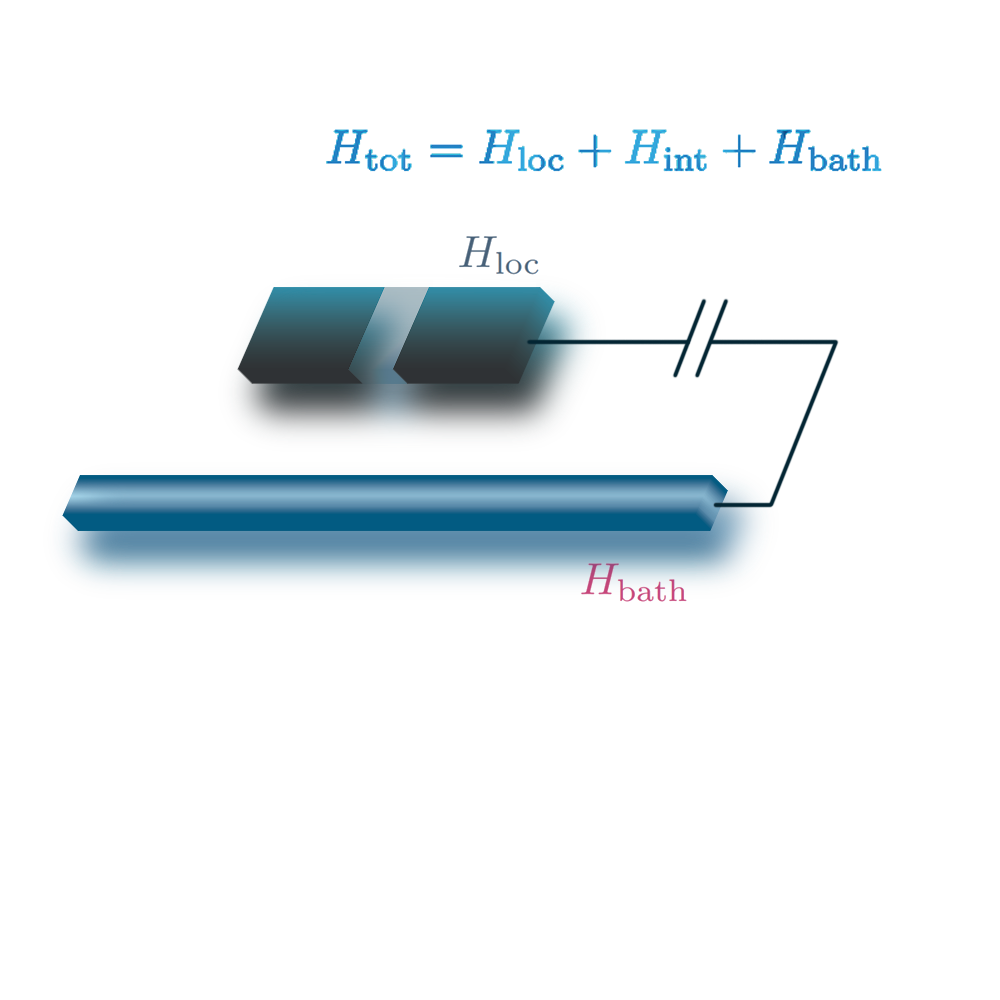
\includegraphics[width=10cm]{TexFigure/Junction_RE.png}}
  \caption{Brief Image of Resistivity shunted Josephson junction}
\end{figure}

\pagebreak
\subsection{Previous work}
A resistively shunted Josephson junction(RSJJ) is a circuit consisting of a single Josephson junction simultaneously 
connected to an RC resonator structure which acts as a circuit resistance. 
Several studies have reported that the Josephson junction in this structure reveals a phase transition scheme 
that depends on the coupling strength between the Junction and the circuit resistance.\cite{"PhysRevB.108.184514"} 
This phenomenon allows RSJJ to play a physical role as a simulator for the quantum phase transition, 
especially for the Schmid quantum dissipative transition. Although RSJJ can be a well-defined physical structure 
for simulating the phase transition, it is limited to zero-temperature conditions, 
which is hard to achieve in an experimental approach.
\subsection{Our approach}
\begin{figure}[htbp]
  \centerline{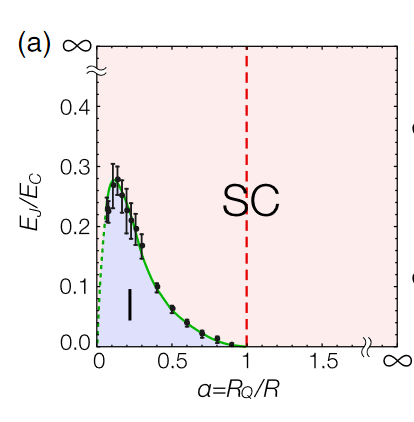
\includegraphics[width=6cm]{TexFigure/kps_INT_exp.PNG}}
  \caption{Zero temperature phase diagram with reentrant phase transition\cite{PhysRevLett.129.087001}}
\end{figure}
In the latest study, a novel phase transition scheme called the ‘reentrant phase transition’ was predicted due to the potential independence of the dispersion relation of the RC resonator. Based on previous research, we’ll investigate this structure in a finite-temperature scheme. We construct the RSJJ Hamiltonian as a pseudo particle impurity model, which is described by the action of system $S$ separated into two parts: for local system $S_{loc}$ and for interaction $S_{int}$, 
\begin{flalign}
  \begin{split}
S = S_{loc} + S_{int}  
\end{split}
\end{flalign}

using Matsubara Green’s function. 

In our model, $S_{loc}$ will be correspond to the dynamics of Josephson junction, and $S_{int}$ will represents the interaction of Josephson junction and the RC resonator.

\end{spacing}

\pagebreak

\section{Theoretical method}
\begin{spacing}{1.5}
\subsection{Circuit model}
\subsubsection*{Hamiltonian of Resistivity shunted Josephson junction}
  \begin{figure}[htbp]
    \centerline{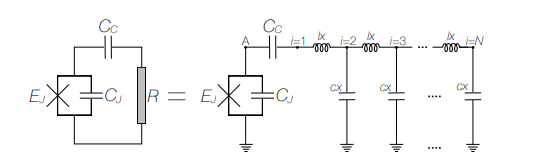
\includegraphics[width=12cm]{TexFigure/circuit_supp_ashida.PNG}}
    \caption{ Picture of resistivity shunted Josephson junction connected with exterior transmission line.\cite{PhysRevLett.129.087001}}
  \end{figure} 
We set the Resistivity shunted Josephson junction(RSJJ) circuit as an impurity model. 
Specific Hamiltonians and physical parameters are based on the ref\cite{PhysRevLett.129.087001}. 
The circuit is composed of a single Josephson junction connected to the transmission line, 
which acts as the resistance of the total circuit system. 
Each component of the circuit is mapped onto each composition of the total Hamiltonian. 
The given circuit Hamiltonian form is represented as follows : 
\begin{flalign}
  \begin{split}
H_{sys} = (E_c\hat{N^2}-E_J\cos{\phi})\otimes I -\hat{N}\otimes\sum_{0<k\leq K}\hbar g_k(\hat{b}_k^\dagger + \hat{b}_k) + I \otimes \sum_{0<k\leq K}\hbar\omega_k\hat{b_k}^\dagger\hat{b_k}
\end{split}
\end{flalign}
Introducing briefly, our target circuit Hamiltonian can be divided into three parts:
\begin{flalign}
  \begin{split}
H_{\text{loc}}+H_{\text{int}}+H_{\text{bath}}
\end{split}
\end{flalign}
Where 
\begin{flalign}
  \begin{split}
H_{\text{loc}} &=E_C\hat{N}^2 - E_J \cos{\phi} \\ H_{\text{bath}} &= \sum_{0<k\leq K} \hbar \omega_k \hat{b}^\dagger_k \hat{b}_k \\ H_{\text{int}} &= -\hat{N}\otimes\sum_{0<k\leq K} \hbar g_k (\hat{b}^\dagger_k + \hat{b}_k)
\end{split}
\end{flalign}
The description of basic symbols is in Table. 1. Here the physical parameter [$\phi,\hat{N}]$ satisfies the commutation relation,
\begin{flalign}
  \begin{split}
[\phi,\hat{N}]=i\hbar
\end{split}
\end{flalign}
$\\$Interaction effect of local(impurity) system between bath is described through  
$g_k$ and the parameter $\alpha =\frac{R_Q}{R}$ .  We use $\alpha$ and $\gamma = \frac{E_J}{E_C}$ 
as parameters to control the criticality of the Josephson junction. We’ve set $E_C$ and $\hbar$ as energy units, 
1 as the value of each parameter during the calculation process. Detailed description of basic symbols is in Table. 1. 
\begin{table}[htbp]
  \centering
  \renewcommand{\arraystretch}{1.2}
  \begin{tabular}{@{}ccc@{}}
  \toprule
  \textbf{Symbols} & \textbf{Formula} & \textbf{Physical quantities} \\ 
  \midrule
  $\phi$ & & Phase of Josephson junction \\ 
  $\hat{N}$ & $-i\frac{\partial}{\partial \phi}$ & Charge operator \\ 
  $\omega_k$ & $vk =\frac{vm\pi}{L}$ & Bath frequency \\ 
  $\hat{b_k}^\dagger,\hat{b_k}$ & & Bosonic creation, annihilation operator \\
  $R_Q$ & $\frac{h}{4e^2}$ & Quantum resistance of junction \\
  $R$ & & Resistance of bath \\
  $E_C$ & $\frac{(2e)^2}{2C_J}$ & Josephson junction charging energy \\ 
  $E_J$ & & Josephson coupling energy \\ 
  $g_k$ & $\sqrt{\frac{2\pi v}{\alpha L} \frac{\omega_k}{1+(\frac{\nu \omega_k}{W})^2}}$ & Coupling with bath in mode $k$ \\ 
  $\nu$ & $\frac{\pi}{\alpha \epsilon_C}$ & \\
  $\epsilon_C$ & $\frac{E_C}{\hbar W}$ & \\
  \bottomrule
  \end{tabular}
  \caption{Basic symbols used for describing Hamiltonian.}
  \end{table}
\subsubsection*{Span of $H_{\text{loc}}$ in Josephson effect basis}
To adjust the expansion method to the RSJJ Hamiltonian model, We represent the local system Hamiltonian in matrix formulation using the Josephson wave function as its basis. We adopt the macroscopic point of view to observe the superconducting effect expected in our junction system. The free-particle basis in exponential form is written as : 
\begin{flalign}
  \begin{split}
\ket{\psi_{JJ}} = \sum_{-\infty}^{\infty} c_me^{im\phi}
\end{split}
\end{flalign}
Here, $c_m$ and $m$ indicates the normalization factor and wave number which analogous to energy excitations. In trigonometric form, it turns out : 
\begin{flalign}
  \begin{split}
\ket{\psi_{JJ}}=\sum_{m=0}^\infty a_m\cos{m\phi} +b_m\sin{m\phi}
\end{split}
\end{flalign}
Where $a_m$ and $b_m$ are the normalization factor corresponds to even and odd trigonal function. separating in odd and even function,
\begin{flalign}
  \begin{split}
\text{even part of the basis} : \sum_{m=0}^\infty a_m\cos{m\phi}\\\text{odd part of the basis} : \sum_{n=1}^\infty b_n\sin{n\phi}
\end{split}
\end{flalign}
In a Hamiltonian of a system with arbitrary dimensions, the eigenvector written in the form of an even function in form of series expansion:
\begin{flalign}
  \begin{split}
\ket{\text{even}_k}=\frac{a^{(k)}_0}{\sqrt{2\pi}} + \sum_{n=1}\frac{a^{(k)}}{\sqrt{\pi}}\cos{n\phi}
\end{split}
\end{flalign}
Here, (k) represents the k-th split state, that is, the energy state of the even function basis split by external perturbation in the k-th excited state. In the same way, the eigenvector written in the form of an odd function is as follows: 
\begin{flalign}
  \begin{split}
\ket{\text{odd}_k} = \sum_{m=1}\frac{b_m^{(k)}}{\sqrt{\pi}}\sin{m\phi}
\end{split}
\end{flalign}
And its matrix form is : 
\begin{flalign}
  \begin{split}
\ket{\text{even}_k}=\begin{pmatrix} \alpha_0 \\ \alpha_1\\ \vdots \\\alpha_m\end{pmatrix}\quad, \quad \ket{\text{odd}_k}=\begin{pmatrix} \beta_1 \\ \beta_2\\ \vdots \\\beta_m\end{pmatrix}
\end{split}
\end{flalign}
We can span the target Hamiltonian in given basis.Considering the differential form of local system Hamiltonian with using above result,  
\begin{flalign}
  \begin{split}
H_{\text{loc}} = -\frac{\partial^2}{\partial \phi^2} - \gamma\cos{\phi}
\end{split}
\end{flalign}

\begin{flalign}
  \begin{split}
&H_{\text{loc}}\ket{\psi_{JJ}} = H_{\text{loc}}(\ket{\text{even}_k}+\ket{\text{odd}_k}) \\ \text{ } 
\\ &\bigg(-\frac{\partial^2}{\partial \phi^2} - \gamma\cos{\phi}\bigg)\bigg(\sum_{m=0}^\infty a_m\cos{m\phi} +\sum_{n=1}^\infty b_n\sin{n\phi}\bigg) 
\\&= -\sum_{m=0}^\infty (m^2a_m\cos{m\phi}+\gamma\cos{\phi}\cos{m\phi})-\sum_{n=1}^\infty (n^2b_n\sin{n\phi}+\gamma\cos{\phi}\sin{n\phi})
\end{split}
\end{flalign}
In matrix representation,
\begin{flalign}
  \begin{split}
H_{\text{loc even}} = \begin{pmatrix}
0 & -\frac{\gamma}{\sqrt{2}} & 0 & \cdots \\
-\frac{\gamma}{\sqrt{2}} & 1 & -\frac{\gamma}{2} & 0 & \cdots \\ &  \\
0 & -\frac{\gamma}{2} & 4 &  \\
\vdots &  &  & \ddots 
\end{pmatrix}
\qquad (m = 0,1,2, \dots)
\end{split}
\end{flalign}

\begin{flalign}
  \begin{split}
H_{\text{loc odd}} = \begin{pmatrix}
1 & -\frac{\gamma}{2} & 0 & \cdots \\
-\frac{\gamma}{2} & 4 & -\frac{\gamma}{2} & 0 & \cdots \\ &  \\
0 & -\frac{\gamma}{2} & 9 &  \\
\vdots &  &  & \ddots 
\end{pmatrix}
\qquad (m = 1,2, \dots)
\end{split}
\end{flalign}

To study how system changes depends on coupling parameters and finite temperature conditions, we measure the total RSJJ Hamiltonian under local system basis engaged from diagonalization of the $H_{\text{loc even}}$ and $H_{\text{loc odd}}$ . 
\subsubsection*{Matrix form of $\hat{N}$  in local basis}
The charge operator $\hat{N}$ pursues polarization operator in our expansion model, endows coupling effect between local system and bath system. Exploiting local basis from previous procedure, We can write $\hat{N}$ in aspect of local system view.
\subsubsection*{2-level case}
Now, we can span the charge operator in eigenvectors of $H_{\text{loc even}}$ and $H_{\text{loc odd}}$. In 2-level case, we can use total lowest three states as basis vector,
\begin{flalign}
  \begin{split}
&\ket{\text{gs}}=\frac{a^{(0)}_0}{\sqrt{2\pi}} + \sum_{n=1}\frac{a^{(0)}_n}{\sqrt{\pi}}\cos{n\phi} = \frac{a_0}{\sqrt{2\pi}} + \frac{a_1}{{\sqrt{\pi}}}\cos{\phi} + \frac{a_2}{\sqrt{\pi}} \cos{2\phi} +\cdots\\
&\ket{\text{1st}} = \sum_{m=1}\frac{b^{(1)}_m}{\sqrt{\pi}}\sin{m\phi} = \frac{b_1}{{\sqrt{\pi}}}\sin{\phi} +  \frac{b_2}{\sqrt{\pi}} \sin{2\phi}+\cdots\\
&\ket{\text{2nd}}=\frac{a^{(1)}_0}{\sqrt{2\pi}} + \sum_{n=1}\frac{a^{(1)}_n}{\sqrt{\pi}}\cos{n\phi}= \frac{a'_0}{\sqrt{2\pi}} + \frac{a'_1}{{\sqrt{\pi}}}\cos{\phi} + \frac{a'_2}{\sqrt{\pi}} \cos{2\phi} +\cdots
\end{split}
\end{flalign}
Here we note the upper indices with round brace to indicate the energy excitation of local system. Then matrix form of $\hat{N}$ becomes :
\begin{flalign}
  \begin{split}
\hat{N} &= \begin{pmatrix}
\bra{\text{gs}}-i\frac{\partial}{\partial\phi}\ket{\text{gs}} & \bra{\text{gs}}-i\frac{\partial}{\partial\phi}\ket{\text{1st}} & \bra{\text{gs}}-i\frac{\partial}{\partial\phi}\ket{\text{2nd}} \\
\bra{\text{1st}}-i\frac{\partial}{\partial\phi}\ket{\text{gs}} &  \bra{\text{1st}}-i\frac{\partial}{\partial\phi}\ket{\text{1st}} & \bra{\text{1st}}-i\frac{\partial}{\partial\phi}\ket{\text{2nd}} \\ 
\bra{\text{2nd}}-i\frac{\partial}{\partial\phi}\ket{\text{gs}} & \bra{\text{2nd}}-i\frac{\partial}{\partial\phi}\ket{\text{1st}} & \bra{\text{2nd}}-i\frac{\partial}{\partial\phi}\ket{\text{2nd}}
\end{pmatrix} \\ \quad \\ 
&=i\begin{pmatrix}
0 & \sum_{n=1}na^{(0)}_n b^{(1)}_n & 0\\
-\sum_{n=1}na^{(0)}_n b^{(1)}_n &  0 & -\sum_{n=1}na^{(1)}_n b^{(1)}_n \\ 
0 & \sum_{n=1}na^{(1)}_n b^{(1)}_n & 0
\end{pmatrix}
\end{split}
\end{flalign}
\subsubsection*{Multilevel case}
For a 2-level system (without considering energy level splitting; the energy level needs to be split by external perturbation to become a 3-level Hamiltonian) or higher, the process of expressing the order parameter in matrix form for the Hamiltonian $H_{\text{loc}}$ of the system under consideration involves the following steps.
Now based on the above discussion, the extended form of charge operator in higher dimension is :
\begin{flalign}
  \begin{split}
\hat{N} &= \begin{pmatrix}
\bra{\text{gs}}-i\frac{\partial}{\partial\phi}\ket{\text{gs}} & \bra{\text{gs}}-i\frac{\partial}{\partial\phi}\ket{\text{1st}} & \cdots \\
\bra{\text{1st}}-i\frac{\partial}{\partial\phi}\ket{\text{gs}} &  \ddots & \vdots \\ 
\vdots & \cdots & \bra{\text{nth}}-i\frac{\partial}{\partial\phi}\ket{\text{nth}}
\end{pmatrix} \\ \quad \\ 
&=i\begin{pmatrix}
0 & \sum_{n=1}na^{(0)}_n b^{(1)}_n & \cdots \\
-\sum_{n=1}na^{(0)}_n b^{(1)}_n &  \ddots & \ \\ & &-\sum_{n=1}na^{(n-1)}_n b^{(n)}_n \\ 
\vdots & \sum_{n=1}na^{(n-1)}_n b^{(n)}_n & 
\end{pmatrix}
\end{split}
\end{flalign}
$\\$
In this case, the maximum dimension of $\hat{N}$  is $2n+1$ .
\pagebreak
\subsubsection*{Matrix Form of $\hat{\cos\phi}$}
The physical observable $\hat{\cos\phi}$ represents the phase coherence of the currents flowing at both ends of the Josephson junction. 
If the junction exhibits superconducting properties, the value of $\hat{\cos\phi}$ will be greater than 0, 
while it will be close to 0 if it exhibits insulating properties.
The expectation of order parameter can be calculated in following formula:
\begin{flalign}
  \begin{split}
  \langle \cos\phi\rangle = \frac{\text{Tr}[\hat{\cos\phi}e^{\beta H}]}{\text{Tr}[e^{-\beta H}]}
\end{split}
\end{flalign}
\subsubsection*{2-level case}
Since we aim to understand the system from the perspective of which represents the Josephson junction with three energy levels, 
we intend to expand order parameter $\cos \phi$ in simliar procedure with calculating $\hat{N}$ matrix. Adopting the form of fourier basis 
in the case of 2-level in the representing $\hat{N}$ matrix, $\cos\phi$ can be rewritten as a matrix operator, and 
\begin{flalign}
  \begin{split}
\hat{\cos{\phi}} = \begin{pmatrix}
\bra{\text{gs}}\cos{\phi} \ket{\text{gs}} & \bra{\text{gs}}\cos{\phi}\ket{\text{1st}} & \bra{\text{gs}}\cos{\phi}\ket{\text{2nd}}  \\
\bra{\text{1st}}\cos{\phi}\ket{\text{gs}} & \bra{\text{1st}}\cos{\phi}\ket{\text{1st}} & \bra{\text{1st}}\cos{\phi}\ket{\text{2nd}}  \\
\bra{\text{2nd}}\cos{\phi}\ket{\text{gs}} & \bra{\text{2nd}}\cos{\phi}\ket{\text{1st}} & \bra{\text{2nd}}\cos{\phi}\ket{\text{2nd}} \\
\end{pmatrix} 
\end{split}
\end{flalign}
When obtaining eigenvectors for the 2-level truncated 3*3 $H_{\text{loc}}$ matrix, the matrix form of $\cos\phi$ is expressed as follows.
\begin{flalign}
  \begin{split}
\hat{\cos{\phi}} = \begin{pmatrix}
\frac{2}{\sqrt{2}}a_0a_1 + a_1a_2 & 0 & \frac{1}{\sqrt{2}}(a_1a'_0 + a_0a'_1) + \frac{1}{2}(a_1a'_2 + a_2a'_1)  \\
0 & b_1b_2 & 0  \\
\frac{1}{\sqrt{2}}(a_1a'_0 + a_0a'_1) + \frac{1}{2}(a_1a'_2 + a_2a'_1) & 0 & \frac{2}{\sqrt{2}}a'_0a'_1 + a'_1a'_2 \\
\end{pmatrix} 
\end{split}
\end{flalign}
$\\$
\subsubsection*{Multilevel case}
For a 2-level system (without considering energy level splitting; the energy level needs to be split by external perturbation to become a 3-level Hamiltonian) or higher, the process of expressing the order parameter in matrix form for the Hamiltonian $H_{\text{loc}}$ of the system under consideration involves the following steps.
First, the calculation of the even function form of the order parameter $\cos \phi$ is as follows:
\begin{flalign}
  \begin{split}
\cos{\phi} \ket{\text{even}_k} = \frac{a^{(k)}_0}{\sqrt{2\pi}}\cos{\phi} + \sum_{n=1}\frac{a^{(k)}}{\sqrt{\pi}}\cos{\phi}\cos{n\phi}
\end{split}
\end{flalign}
And Final innerproduct result is:
\begin{flalign}
  \begin{split}
\bra{\text{even}_l}\cos{\phi} \ket{\text{even}_k} = \int^{2\pi}_0\bigg(\frac{a^{(m)}_0}{\sqrt{2\pi}} + \sum_{m=1}\frac{a^{(m)}}{\sqrt{\pi}}\cos{m\phi}\bigg)\bigg(\frac{a^{(n)}_0}{\sqrt{2\pi}}\cos{\phi} + \sum_{n=1}\frac{a^{(n)}}{\sqrt{\pi}}\cos{\phi}\cos{n\phi}\bigg)
\end{split}
\end{flalign}
The calculation for the odd function form is as follows:
\begin{flalign}
  \begin{split}
\ket{\text{odd}}=\sum_{n=1} \frac{b_n^{(k)}}{\sqrt{\pi}}\sin{n\phi} \quad , \quad
\cos{\phi}\ket{\text{odd}}=\sum_{n=1}\frac{b_n^{(k)}}{\sqrt{\pi}}\cos{\phi}\sin{n\phi}
\end{split}
\end{flalign}
Similar with the case of even state eigenvector, innerproduct result is:
\begin{flalign}
  \begin{split}
    &\bra{\text{odd}_l}\cos{\phi} \ket{\text{odd}_k} = \sum_{n,m=1}\int^{2\pi}_0 d\phi \bigg(\frac{b_n^{(k)}b_m^{(l)}}{\pi}\cos{\phi}\sin{n\phi}\sin{m\phi}\bigg) \\
    &=    \left\{
        \begin{array}{ll}
            \text{if k} < \text{l : }  \qquad \sum^N_{n=1} \bigg(\frac{\hat{b}^{(k)}_n\hat{b}^{(l)}_{n-1}}{2} + \frac{\hat{b}^{(k)}_n\hat{b}^{(l)}_{n+1}}{2}\bigg)\\
            \text{if k } > \text{l : }  \qquad \sum^N_{n=1} \bigg(\frac{\hat{b}^{(k)}_{n-1}\hat{b}^{(l)}_{n}}{2} + \frac{\hat{b}^{(k)}_{n+1}\hat{b}^{(l)}_{n}}{2}\bigg)
        \end{array}
        \right.
\end{split}
      \end{flalign}
Therefore, when the entire $\cos{\phi}$ is expressed in matrix form, it takes the following form:
\begin{flalign}
  \begin{split}
    \hat{\cos{\phi}} = \begin{pmatrix}
       \ddots & & \vdots & & \\
      & \bra{\text{even}_k}\cos\phi\ket{\text{even}_k} & 0 & \bra{\text{even}_k}\cos\phi\ket{\text{even}_{k+1}} & \cdots \\
      & 0 & \bra{\text{odd}_k}\cos\phi\ket{\text{odd}_k} & 0 & \bra{\text{odd}_k}\cos\phi\ket{\text{odd}_{k+1}} \\
      & \bra{\text{even}_{k+1}}\cos\phi\ket{\text{even}_k} & 0 & \bra{\text{even}_{k+1}}\cos\phi\ket{\text{even}_{k+1}} & \\
      & & \vdots & &\ddots \\
      \end{pmatrix} 
    \end{split}
    \end{flalign}
\end{spacing}
\pagebreak


\subsection{Diagrammatic method}
\subsubsection*{Field operator and Green's function}
\begin{spacing}{1.5}
In this chapter, We will briefly introduce the theoretical framework of the method of Green’s function, and pseudo-particle solvers, such as Non-crossing approximation. 
The detailed mathmatical derivation will treated on appendix.

In quantum many-body theory, the physical system is depicted over the frame of the fermionic(bosonic) creation and annihilation operator, and $\hat{a}(\hat{a}^\dagger)$ as an annihilation(creation) operator, it satisfies the following commutation relations:
\begin{flalign}
  \begin{split}
[\hat{a_i},\hat{a_j}] &= \{\hat{a_i},\hat{a_j}\} = 0 \\ 
[\hat{a_i}^\dagger,\hat{a_j}^\dagger] &= \{\hat{a_i}^\dagger,\hat{a_j}^\dagger\}=0\\ 
[\hat{a_i},\hat{a_j}^\dagger] = \{\hat{a_i},\hat{a_j}^\dagger\} &= \delta_{ij} = \begin{cases} 1 \quad (i=j)\\  0 \quad (i \neq j)\quad \end{cases}
\end{split}
\end{flalign}
Where the square bracket informs the bosonic case, and its RHS indicates the fermionic case. In the following discussion, we will drop out the lower indices of the field operator, assuming it can indicate any arbitrary quantum states.
If we consider the Hamiltonian system can be split into two parts: for the local system and for interaction, we can write the total Hamiltonian $H$:
\begin{flalign}
  \begin{split}
H = H_0 + H_{\text{int}}
\end{split}
\end{flalign}
Here, $H_0$ is the local(Free) Hamiltonian, $H_{\text{int}}$  is the Hamiltonian for interaction (external potential). To express the dynamics of a given operator, we depict the time dependency of the operator in the interaction picture :
\begin{flalign}
  \begin{split}
\hat{a}(t) = e^{iH_0t}\hat{a}e^{-iH_0t} \\ \hat{a}^\dagger(t) =  e^{-iH_0t}\hat{a}^\dagger e^{iH_0t} 
\end{split}
\end{flalign}
With the above time dependency, we can define the Green’s function as follows :
\begin{flalign}
  \begin{split}
G_0(t,t') = \frac{i}{\hbar}\langle \mathcal{T}\hat{a}^\dagger(t)\hat{a}(t')\rangle = \begin{cases} \frac{i}{\hbar}\langle \hat{a}^\dagger(t)\hat{a}(t')\rangle  \quad (t>t')\\  \pm\frac{i}{\hbar}\langle \hat{a}(t')\hat{a}^\dagger(t)\rangle \quad (t<t')\quad \end{cases}
\end{split}
\end{flalign}
Here, the symbol $\mathcal{T}$ is the time ordering operator. One of the features of Green’s function is that it satisfies the given equation of motion :
\begin{flalign}
  \begin{split}
[i \partial_t-H] &G(t,t')=\delta(t-t') \\
[i \partial_t-H_0]G_0(t,t')&=[i \partial_t-H+H']G_0(t,t')=\delta(t-t')
\end{split}
\end{flalign}
\subsubsection*{Diagrammatic expansion of Green’s function}
In the statistical framework, it is easy to calculate Green’s function in the imaginary time $\tau$ due to the wick rotation of the time axis, which mapped time-dependent system progression into thermal equilibrium problems with temperature dependency.
\begin{flalign}
  \begin{split}
\frac{it}{\hbar}=\tau = \beta = \frac{1}{k_BT}
\end{split}
\end{flalign}
We will use $\hbar=1$ in overall discussion. In this new frame, Green’s function can be rewritten :
\begin{flalign}
  \begin{split}
G_0(\tau,\tau') = \langle\mathcal{T}\hat{a}^\dagger(\tau)\hat{a}(\tau)\rangle\begin{cases} \langle \hat{a}^\dagger(\tau)\hat{a}(\tau')\rangle  \quad (\tau>\tau')\\  \pm \langle \hat{a}(\tau')\hat{a}^\dagger(\tau)\rangle \quad (\tau<\tau')\quad \end{cases}
\end{split}
\end{flalign}
There are particular relationship between real-time Green’s function and imaginary time(temperature dependence) Green’s function, which is :
\begin{flalign}
  \begin{split}
G(t,t')\vert_{t=0} = \pm e^{\beta H} G(t,t')\vert_{t=i\beta}
\end{split}
\end{flalign}
These temperature dependence Green’s function is often called as Matsubara Green’s function. 
Single Green’s function corresponding with one specific imaginary time interval can be represented in a diagrammatic way, 
which is the very basic formulation of the diagrammatic method. We can draw a line from $\tau'$  to $\tau$,
\begin{figure}[htbp]
  \centerline{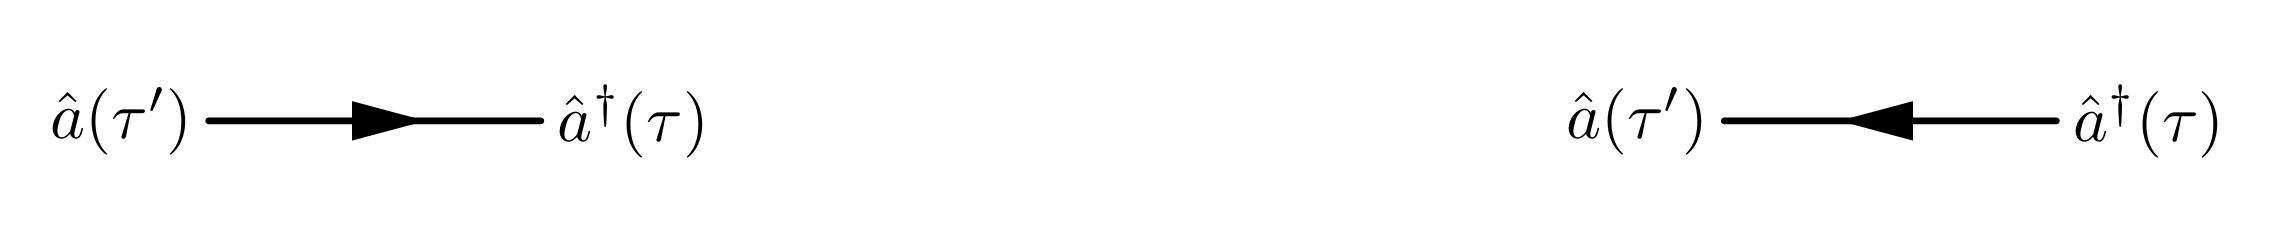
\includegraphics[width=15cm]{TexFigure/Diagram_arrow.PNG}}
  \caption{Diagram of single Green's function. The direction of arrow corresponds with the direction of time flow.}
\end{figure}
\\
In equilibrium statistical mechanics, the expectation value of the physical observable is characterized by the partition function that satisfies the given restricted energy condition in phase space. Based on these concepts, on the grand canonical ensemble, the statistical structure of counting Green’s function becomes :  
\begin{flalign}
  \begin{split}
G_0(\tau,\tau') = \frac{\text{Tr}[e^{-\beta H_0} \hat{a}^\dagger(\tau)\hat{a}(\tau')]}{\text{Tr}[e^{-\beta H_0}]} =\frac{\text{Tr}[e^{-\beta H_0} e^{iH_0 \tau} \hat{a}^\dagger e^{-H_0 (\tau-\tau')}\hat{a}e^{-iH_0 \tau'}]}{\text{Tr}[e^{-\beta H_0}]}
\end{split}
\end{flalign}
This is the very basic form of Green’s function in imaginary time corresponding to the diagram structure. Similar case with the creation and annihilation operator, the time dependency of external potential term Hamiltonian : 
\begin{flalign}
  \begin{split}
H'(\tau) = e^{H_0\tau}He^{-H_0\tau}
\end{split}
\end{flalign}
If we consider the effect of interaction, we can adopt full Green’s function includes the interaction operator $U(\tau)$,
\begin{flalign}
  \begin{split}
G(\tau,\tau') = \frac{\text{Tr}[e^{-\beta H_0} U(\beta)\hat{a}^\dagger(\tau)\hat{a}(\tau')]}{\text{Tr}[e^{-\beta H_0}U(\beta)]} =\frac{\text{Tr}[e^{-\beta H} U(\tau) \hat{a}^\dagger U(\tau'-\tau)\hat{a}U(\tau')]}{\text{Tr}[e^{-\beta H}]} 
\end{split}
\end{flalign}
where interaction operator is : 
\begin{flalign}
  \begin{split}
U(\tau) = \mathcal{T}e^{-\int^\tau_0 d\tau' H_{\text{int}}(\tau')}
\end{split}
\end{flalign}
In the imaginary time interval $[\tau,0]$ , full Green’s function in the expectation form can be represented , 
\begin{flalign}
  \begin{split}
G(\tau,0) = \frac{\text{Tr}[e^{-\beta H_0} U(\beta)\hat{a}^\dagger(\tau)\hat{a}]}{\text{Tr}[e^{-\beta H_0}U(\beta)]} = \frac{\langle U(\beta)\hat{a}^\dagger(\tau)\hat{a}\rangle_0}{\langle U(\beta)\rangle_0}
\end{split}
\end{flalign}
The under index 0 of angled bracket indicates its expectation value was calculated in $H_{\text{loc}}$ frame. If the interaction hamiltonian is in the form of multiplication of pair of annihilation-creation operator $\hat{a}^\dagger$ and $\hat{a}$ , we can adjust Wick’s theorem to expand the each of the expectation value in denominator and numerator into a multiplication of Green’s functions in each time interval. For example, if 
\begin{flalign}
  \begin{split}
H_{\text{int}} =V_{ijkl}\hat{a}^\dagger_i\hat{a}^\dagger_j\hat{a}_k\hat{a}_l
\end{split}
\end{flalign}
Here the term $V_{ijkl}$ is the scalar value (or function) that represents the interaction effect. then 
\begin{flalign}
  \begin{split}
\langle U(\beta)\rangle_0 \sim 1-\frac{1}{2}V_{ijkl}\int^\beta_0d\tau_1\langle\mathcal{T}\hat{a}^\dagger_i(\tau_1)\hat{a}_j^\dagger(\tau_1)\hat{a}_k(\tau_1)\hat{a}_l(\tau_1)\rangle + ... \\=1 - \frac{1}{2}\int^\beta_0\langle\mathcal{T}\hat{a}^\dagger_i(\tau_1)\hat{a}_j^\dagger(\tau_1)\rangle \langle\mathcal{T}\hat{a}_k(\tau_1)\hat{a}_l(\tau_1)\rangle + ...
\end{split}
\end{flalign}
This kind of form of expansion represents the expectation value of the interaction operator in the multiplication of diagrams.
A more detailed discussion will be treated in the Appendix.
\pagebreak
\subsubsection*{Diagrammatic Hybridization expansion in strong coupling case}
In this section, we will introduce the hybridization method based on the former discussion. 
The basic notation and mathematical structure follow the reference[].
The Hamiltonian system can be divided into three parts as a general case of the time-dependent impurity model with a bosonic bath:
\begin{flalign}
  \begin{split}
    H_{sys} = H_{loc}+H_{int}+H_{bath}
  \end{split}
\end{flalign}
In the second quantized form, This can be rewritten:
\begin{flalign}
  \begin{split}
H(t) = H_{loc}(t) + \underbrace{\sum_n \epsilon_n \hat{b}^\dagger_n}_\text{bath} \hat{b}_n + \underbrace{\sum_{m,n} [V_{m,n}(t) c_m^\dagger b_n + \text{H.c.}]}_\text{interaction}
\end{split}
\end{flalign}
The operator $\hat{b} (\hat{b}^\dagger)$  indicates bosonic annihilation(creation) operator, $\hat{c}(\hat{c}^\dagger)$ is fermionic annihilation(creation) operator. 
What we need to focus on is that applying Wick’s theorem isn’t available due to the interaction term, 
which does not pair the same field operator. Based on this structure, the hybridization expansion method was constructed. 
Continue, from the Hamiltonian, the action of the full system can be written into :
\begin{flalign}
  \begin{split}
S = \int^\beta_0 d\tau H_{\text{loc}}(\tau) + \int^\beta_0 d\tau d\tau' P(\tau)\mathcal{W}(\tau-\tau')P(\tau')
\end{split}
\end{flalign}
Here, $H_{\text{loc}}$is the Hamiltonian of the local system, indicating the impurity that we want to focus on. The terms $P$ and $\mathcal{W}$ correspond with the Hermitian operator and the interaction term can be assumed as $\mathcal{W}$ in the previous section.  As we treat the interaction Hamiltonian in the previous section, the term $\mathcal{W}$ includes the scalar factor to represent the effect of the bosonic bath. 
With similar procedure with the diagram expansion, We can calculate the expectation value of observable using the partition function $Z$,
\begin{flalign}
  \begin{split}
Z=\text{tr}\bigg[T_{\tau}e^{-S}\bigg]
\end{split}
\end{flalign}
And in the given frame, the expectation value of observable $O$ can be measured as 
\begin{flalign}
  \begin{split}
\langle T_\tau O(\tau)\rangle = \frac{\text{tr}[T_{\tau}e^{-S} O(\tau)]}{\text{tr[}T_{\tau}e^{-S}]}
\end{split}
\end{flalign}
Which has a similiar form of the full Green’s function. Similiar with it’s diagrammatic expansion, the partition function can be expanded to 
\begin{flalign}
  \begin{split}
Z=\sum^{\infty}_{n=0}Z^{(n)}
\end{split}
\end{flalign}
With it’s full expression, 
\begin{flalign}
  \begin{split}
Z=&\sum_{n=0}^\infty \frac{(-1)^n}{n!} \sum_{\pi \in S_{2n}}\int^\beta_0d\tau_1\int^{\tau_1}_0 d\tau_2 \cdots\int^{\tau_{2n-1}}_0 d\tau_{2n}\text{tr}\bigg[U(\beta-\tau_1)PU(\tau_1-\tau_2)P\cdots P U(\tau_{2n})\bigg] \\
&\times\mathcal{W}(\tau_{\pi(1)}-\tau_{\pi(2)})\cdots\mathcal{W}(\tau_{\pi(2n-1)}-\tau_{\pi(2n)})
\end{split}
\end{flalign}
Here, $\pi(m)$  refers that there are permutations and $S_{2n}$ is a set of available permutations for time ordering. The main Idea of the expansion is, that we only consider the certain “partial set” of full permutation, which corresponds with the non-crossing or crossing connected diagrams. Define the new $\bar{\mathcal{W}}$ function, 
\begin{flalign}
  \begin{split}
\bar{\mathcal{W}} = (\mathcal{W}(\tau) + \mathcal{W}(-\tau))
\end{split}
\end{flalign}
And consider the permutation which only restricted on the case of ,
\begin{flalign}
  \begin{split}
\pi(2j-1) < \pi(2j)
\end{split}
\end{flalign}
We can consider the normalization of the partition function using the chemical potential $\lambda$ in a grand canonical ensemble. With the normalization and the above two rules, we can construct the new formula about the expansion of the partition function, which can be rewritten as :
\begin{flalign}
  \begin{split}
\mathcal{G}(\tau) = \sum^{\infty}_{n=0} \mathcal{G}^{(n)}(\tau) = e^{\tau \lambda}Z
\end{split}
\end{flalign}
which is : 
\begin{flalign}
  \begin{split}
\mathcal{G}^{(0)}(\tau) &= \mathcal{G}_{0}(\tau) \\ \mathcal{G}^{(1)} (\tau) &= \int^\beta_0 d\tau_1 \int^{\tau_1}_0 d\tau_2 \bigg[  \mathcal{G}_{i}(\beta-\tau) P \mathcal{G}_{i}(\tau_1 - \tau_2) P\mathcal{G}_{i}(\tau_2)\bigg] \bar{\mathcal{W}}(\tau_1 - \tau_2)\\
\mathcal{G}^{(2)} (\tau) &= \int^\beta_0 d\tau_1 \int^{\tau_1}_0 d\tau_2 \int^{\tau_2}_0 d\tau_3 \int^{\tau_3}_0 d\tau_4 \bigg[  \mathcal{G}_{i}(\beta-\tau) P \mathcal{G}_{i}(\tau_1 - \tau_2)P \mathcal{G}_{i}(\tau_2 - \tau_3)P \mathcal{G}_{i}(\tau_3 - \tau_4) P\mathcal{G}_{i}(\tau_4)\bigg ]\\ &\times \bigg(\bar{\mathcal{W}}(\tau_1 - \tau_2) \bar{\mathcal{W}}(\tau_3 - \tau_4) +\bar{\mathcal{W}}(\tau_1 - \tau_4) \bar{\mathcal{W}}(\tau_2 - \tau_3) +\bar{\mathcal{W}}(\tau_1 - \tau_3) \bar{\mathcal{W}}(\tau_2 - \tau_4) \bigg)
\end{split}
\end{flalign}
The term $\mathcal{G}_i(\tau)$  is a matrix correspond with $U(\tau)$. We'll define the function as a hybridization function, or, interaction function as the same word. 
During the calculation and the diagrams earned from the previous procedure, 
We can collect the irreducible diagrams that cannot be separated into a number of single propagators. 
These diagrams are defined self-energy, described as follows : 
\begin{flalign}
  \begin{split}
\Sigma(\tau) = \sum_{n=1}^{\infty}\Sigma^{(n)}(\tau)
\end{split}
\end{flalign}
and,
\begin{flalign}
  \begin{split}
\Sigma^{(1)}(\tau) &= \bigg[P\mathcal{G}_{i}(\tau)P\bigg]\bar{\mathcal{W}}(\tau) \\ \Sigma^{(2)}(\tau) &= \int^\beta_0d\tau_1\int^{\tau_1}_0d\tau_2 \bigg[P\mathcal{G}_{i}(\tau-\tau_1)P\mathcal{G}_{i}(\tau_1-\tau_2)P\mathcal{G}_{i}(\tau_2)P\bigg](\bar{\mathcal{W}(\tau)}\bar{\mathcal{W}}(\tau_1-\tau_2) + \bar{\mathcal{W}}(\tau-\tau_2)\bar{\mathcal{W}}(\tau_1))
\end{split}
\end{flalign}
Adopting the self-energy in normalized Partition function, we can gain the equation :
\begin{flalign}
  \begin{split}
\mathcal{G} =& \mathcal{G}_{0}(\tau) + \int^\beta_0d\tau_1\int^{\tau_1}_0d\tau_2\mathcal{G}_{i}(\beta-\tau_1)\Sigma(\tau_1-\tau_2)\mathcal{G}^{(2)}(\tau_2) \\ 
&+ \int^{\beta}_0d\tau_1\int^{\tau_1}_0d\tau_2\int^{\tau_2}_0d\tau_3\int^{\tau_3}_0d\tau_4 \mathcal{G}_{i}(\beta-\tau_1)\Sigma(\tau_1-\tau_2)\mathcal{G}_{i}(\tau_2-\tau_3)\Sigma(\tau_3-\tau_4)\mathcal{G}_{i} + ...
\end{split}
\end{flalign}
This form of Dyson equation can be represented into diagram structure. If we define full $\mathcal{G}$ as :
\begin{flalign}
  \begin{split}
\mathcal{G} = \langle\psi_a(\tau)\psi_b^\dagger(\tau')\rangle = \text{Tr}[e^{\beta H}\psi_a(\tau)\psi_b^\dagger(\tau')]
\end{split}
\end{flalign}
Then the diagram of the Dyson equation turns out to Figure.4.
\begin{figure}[H]
  \centerline{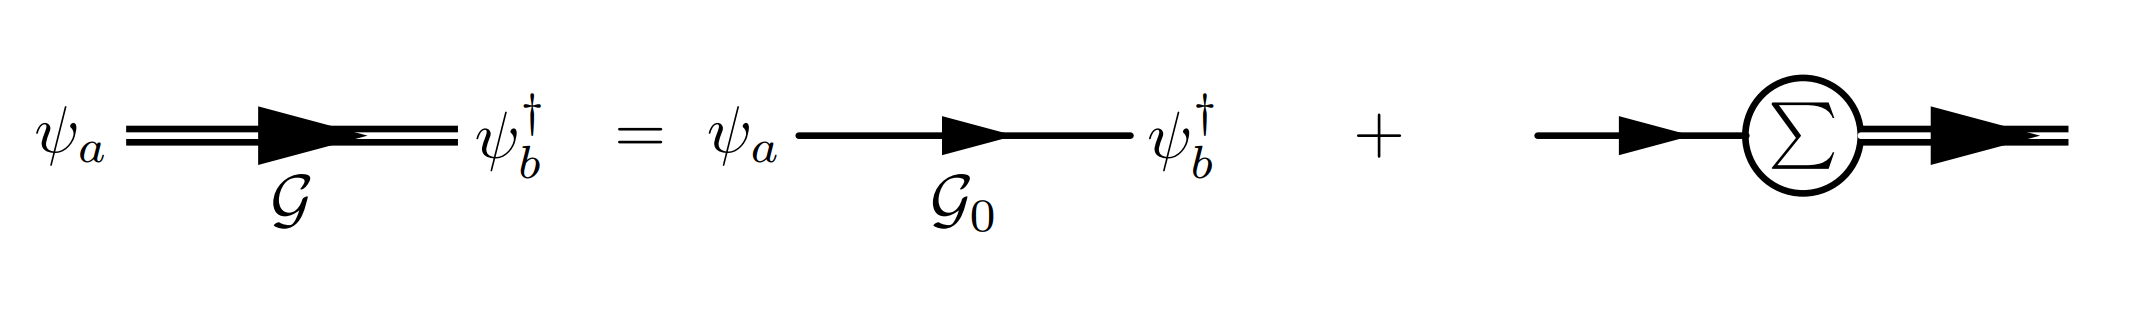
\includegraphics[width=13cm]{TexFigure/Dyson_eq.PNG}}
  \caption{Diagram for Dyson equation with self energy}
\end{figure}
While representing the self-energy in extended diagrammatic formation, we can collect the diagrams with some featured topological structures. For instance, if we consider only the first-order self-energy expansion, the result coincides with the well-known Non-crossing approximation method.
This form of equation satisfies the integral-differential form, agrees with the equation of motion of in the quantum mechanical aspect.
\begin{flalign}
  \begin{split}
[-\partial_{\tau}-H_{\text{loc}}+\lambda]\mathcal{G}(\tau)-\int^\tau_0 d\tau_1\Sigma(\tau-\tau_1)\mathcal{G}(\tau_1) = 0 \quad, \quad(\tau>0)
\end{split}
\end{flalign}
\begin{figure}[H]
  \centerline{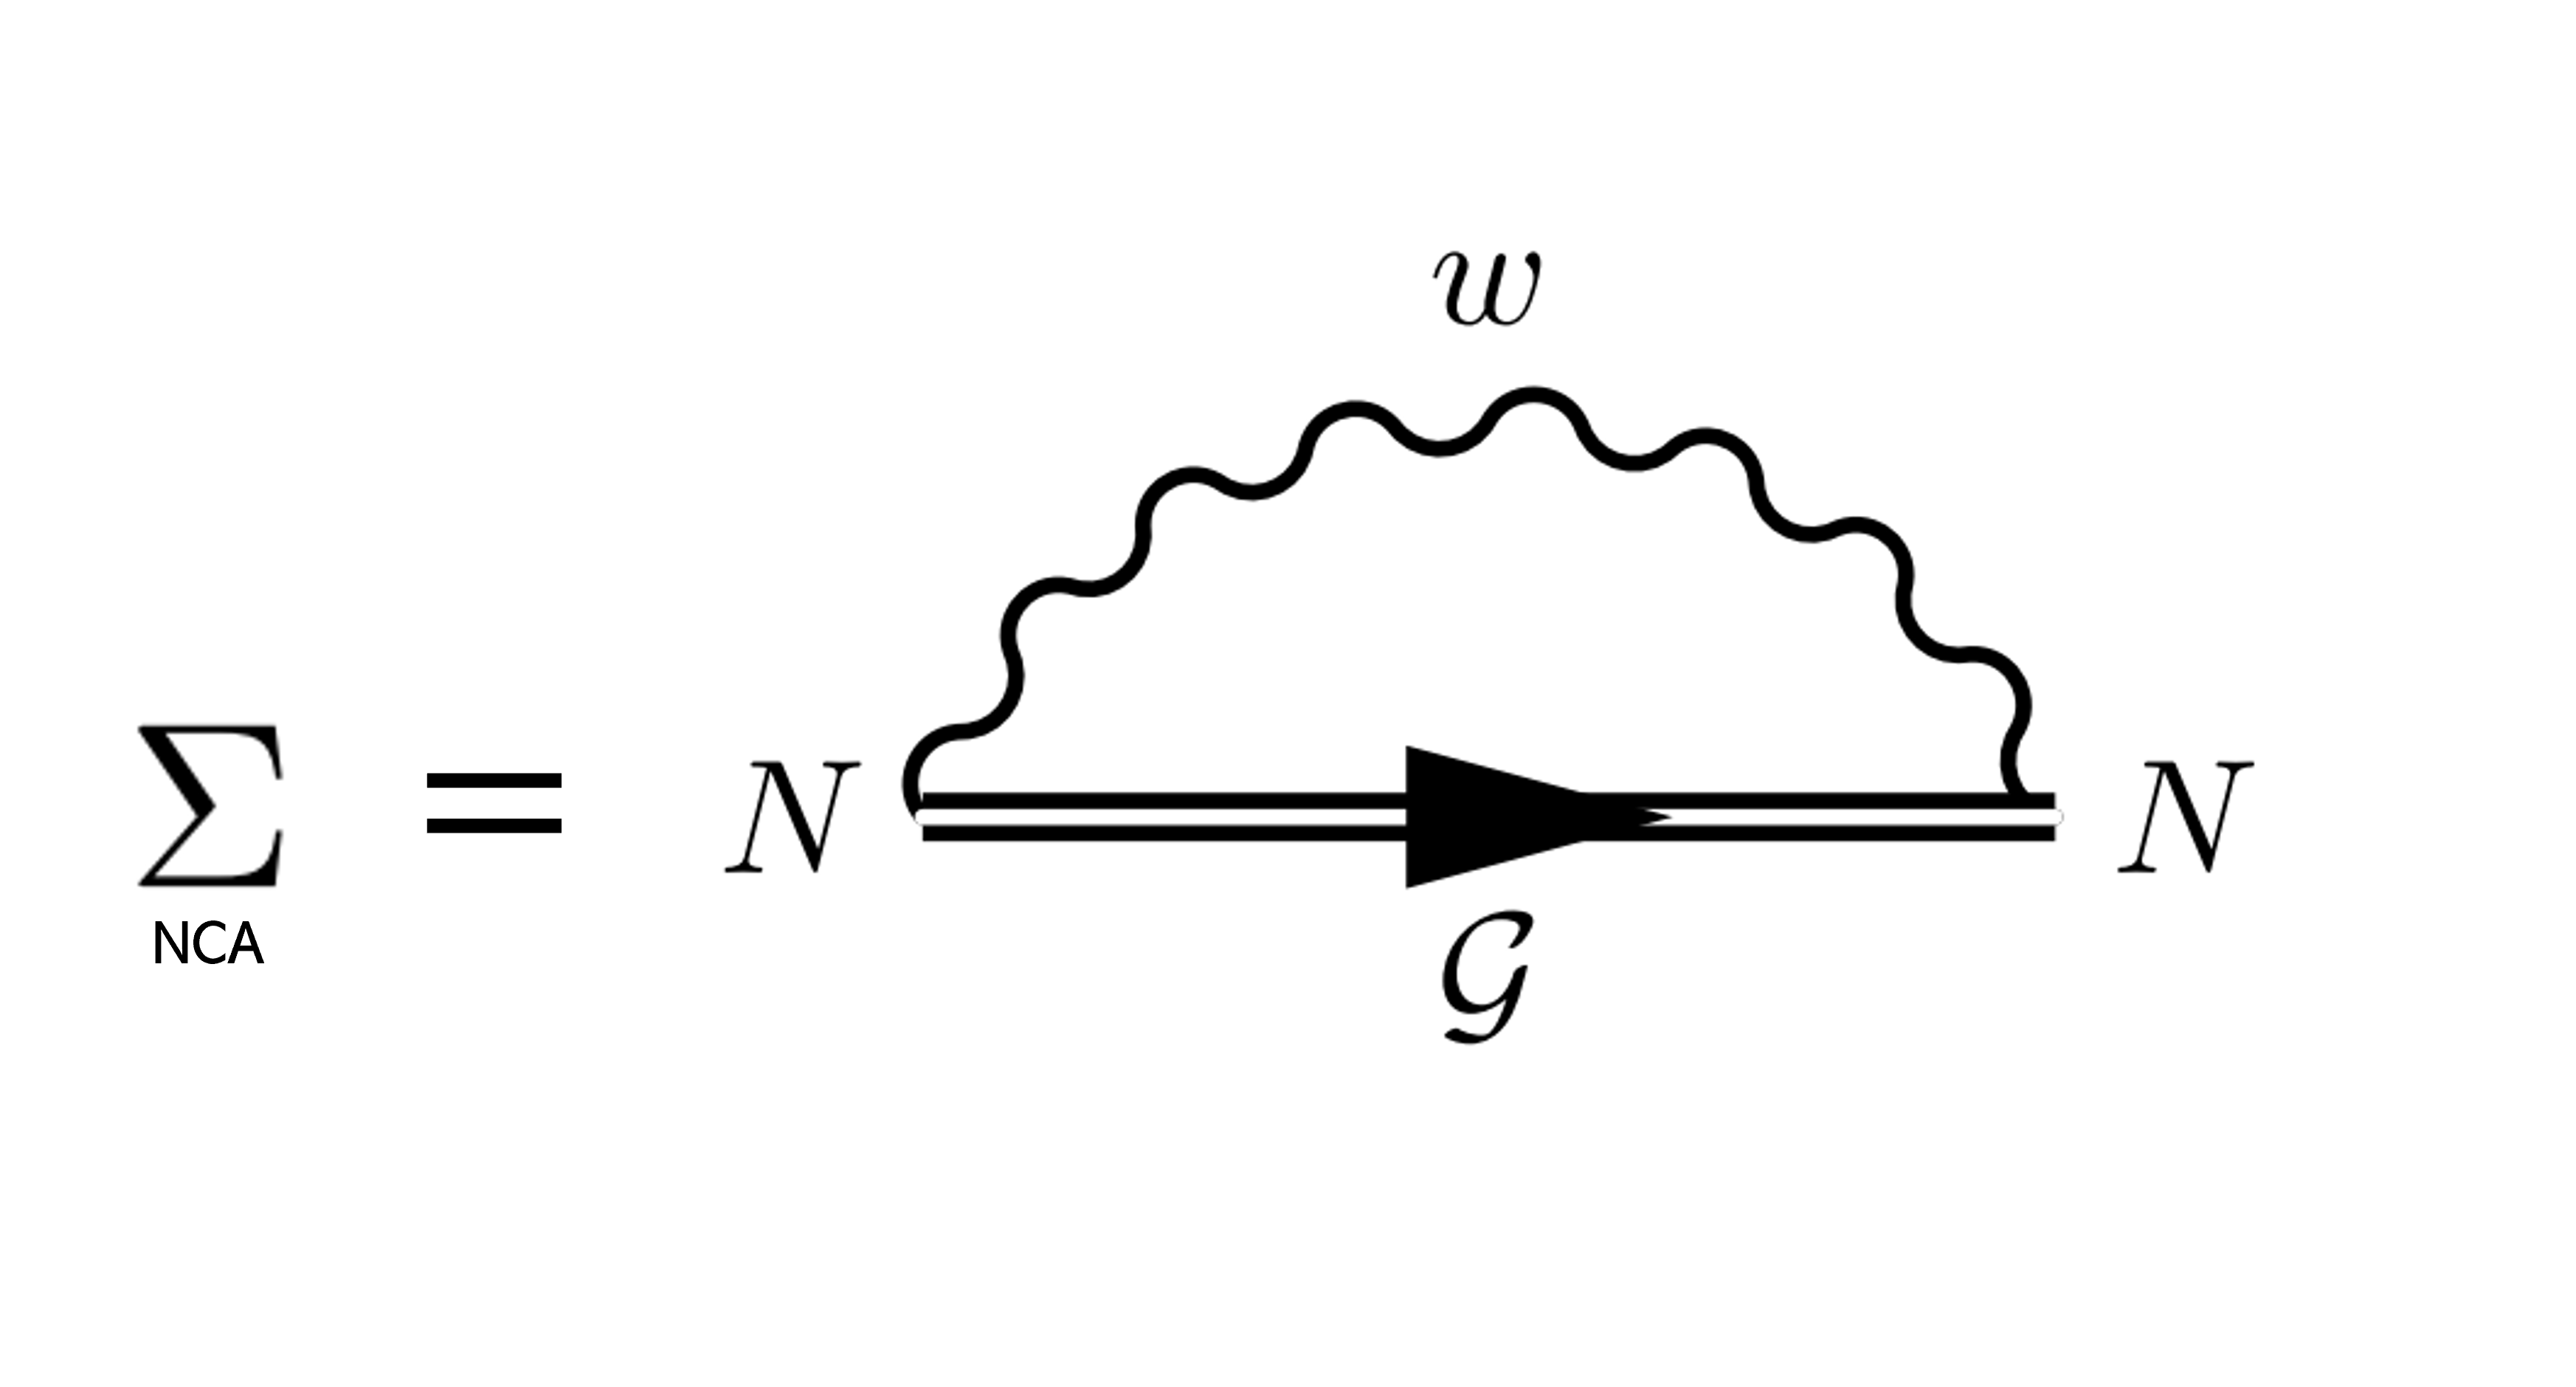
\includegraphics[width=8cm]{TexFigure/NCA_self.PNG}}
  \centerline{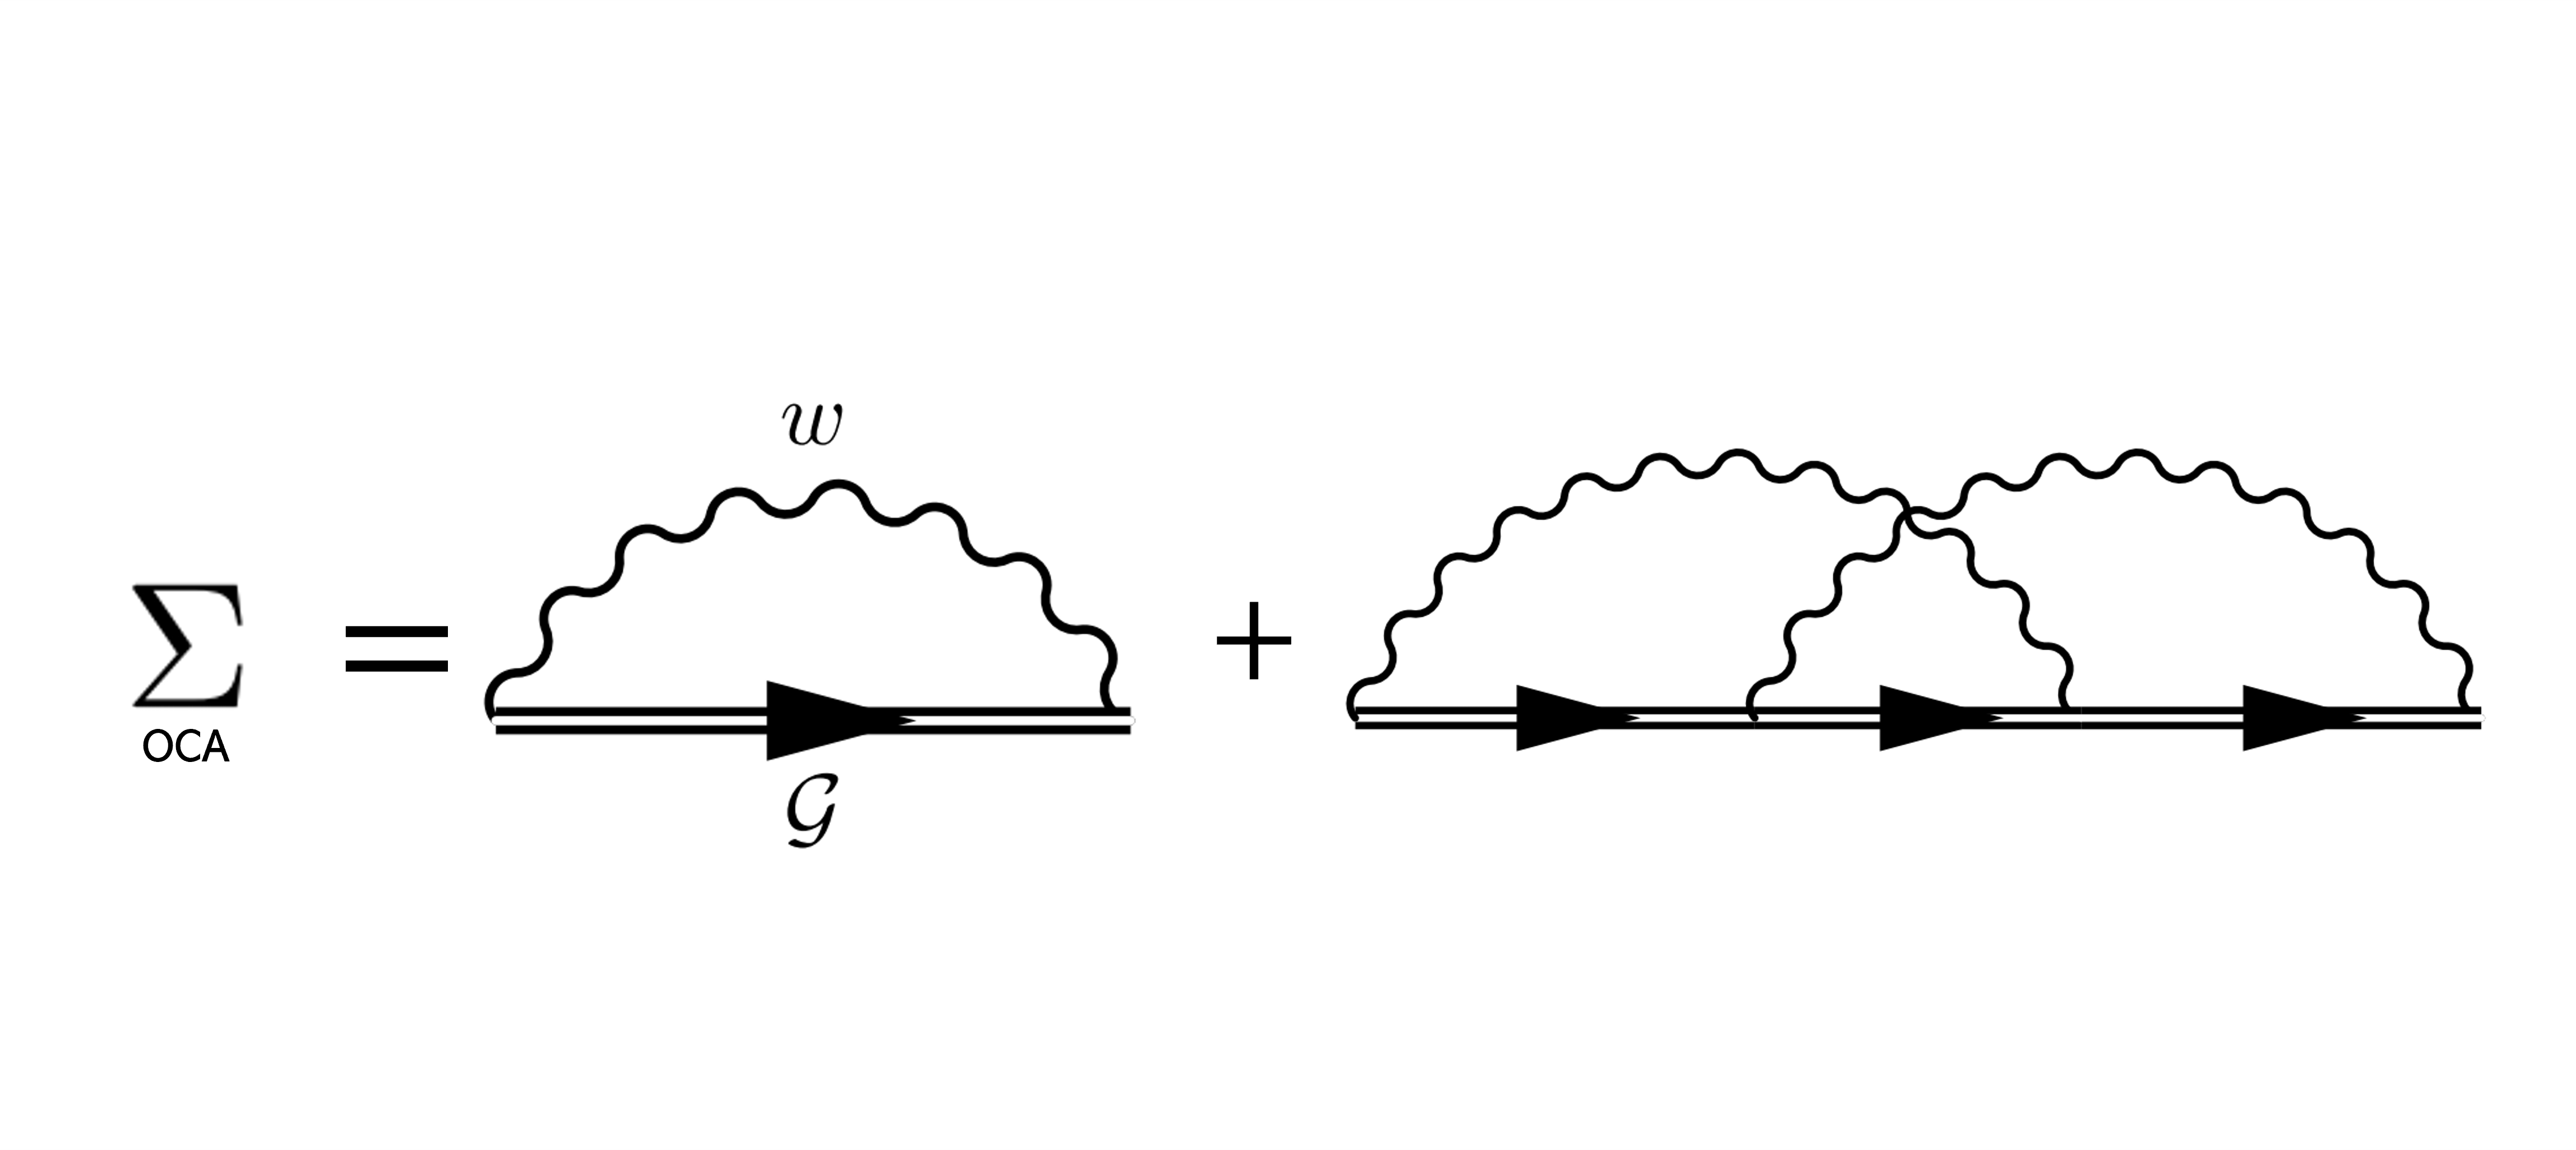
\includegraphics[width=12cm]{TexFigure/OCA_self.PNG}}
  \caption{Self-energy diagram for order of expansion}
\end{figure}
\begin{figure}[H]
  \centerline{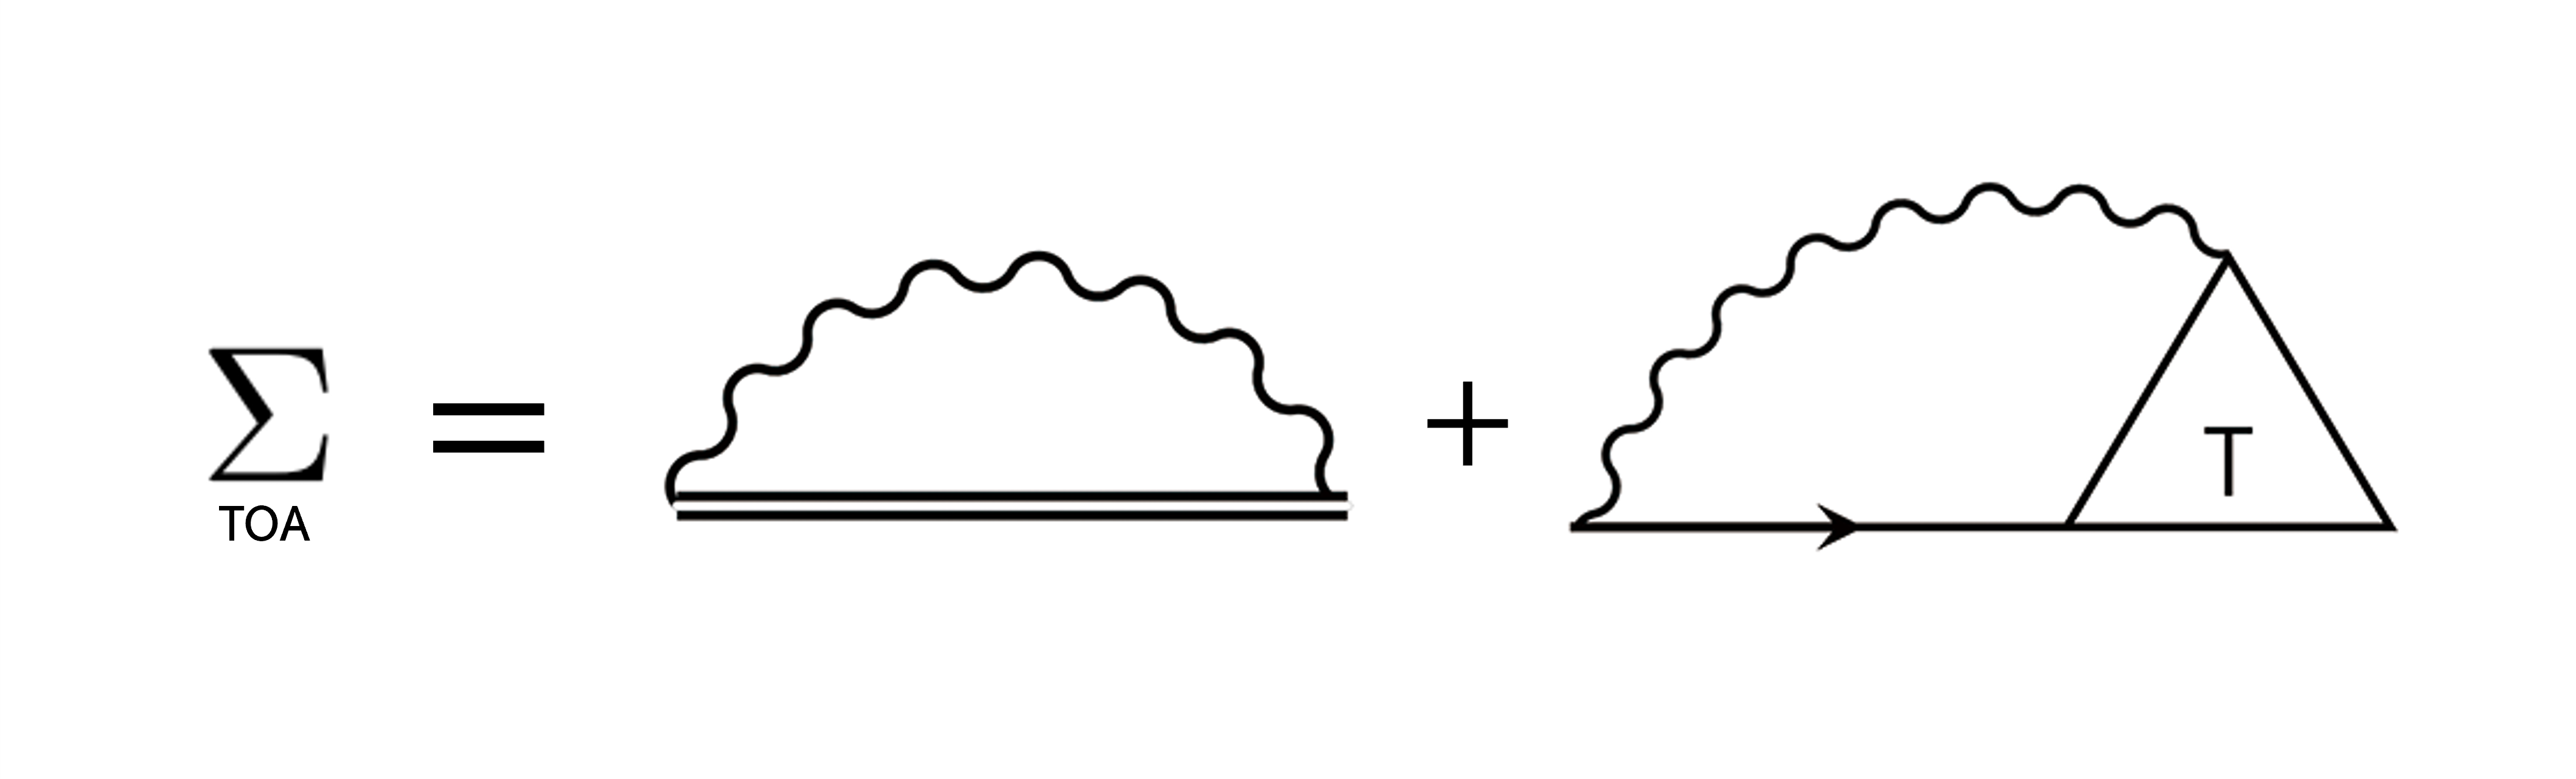
\includegraphics[width=12cm]{TexFigure/TOA_se.png}}
  \centerline{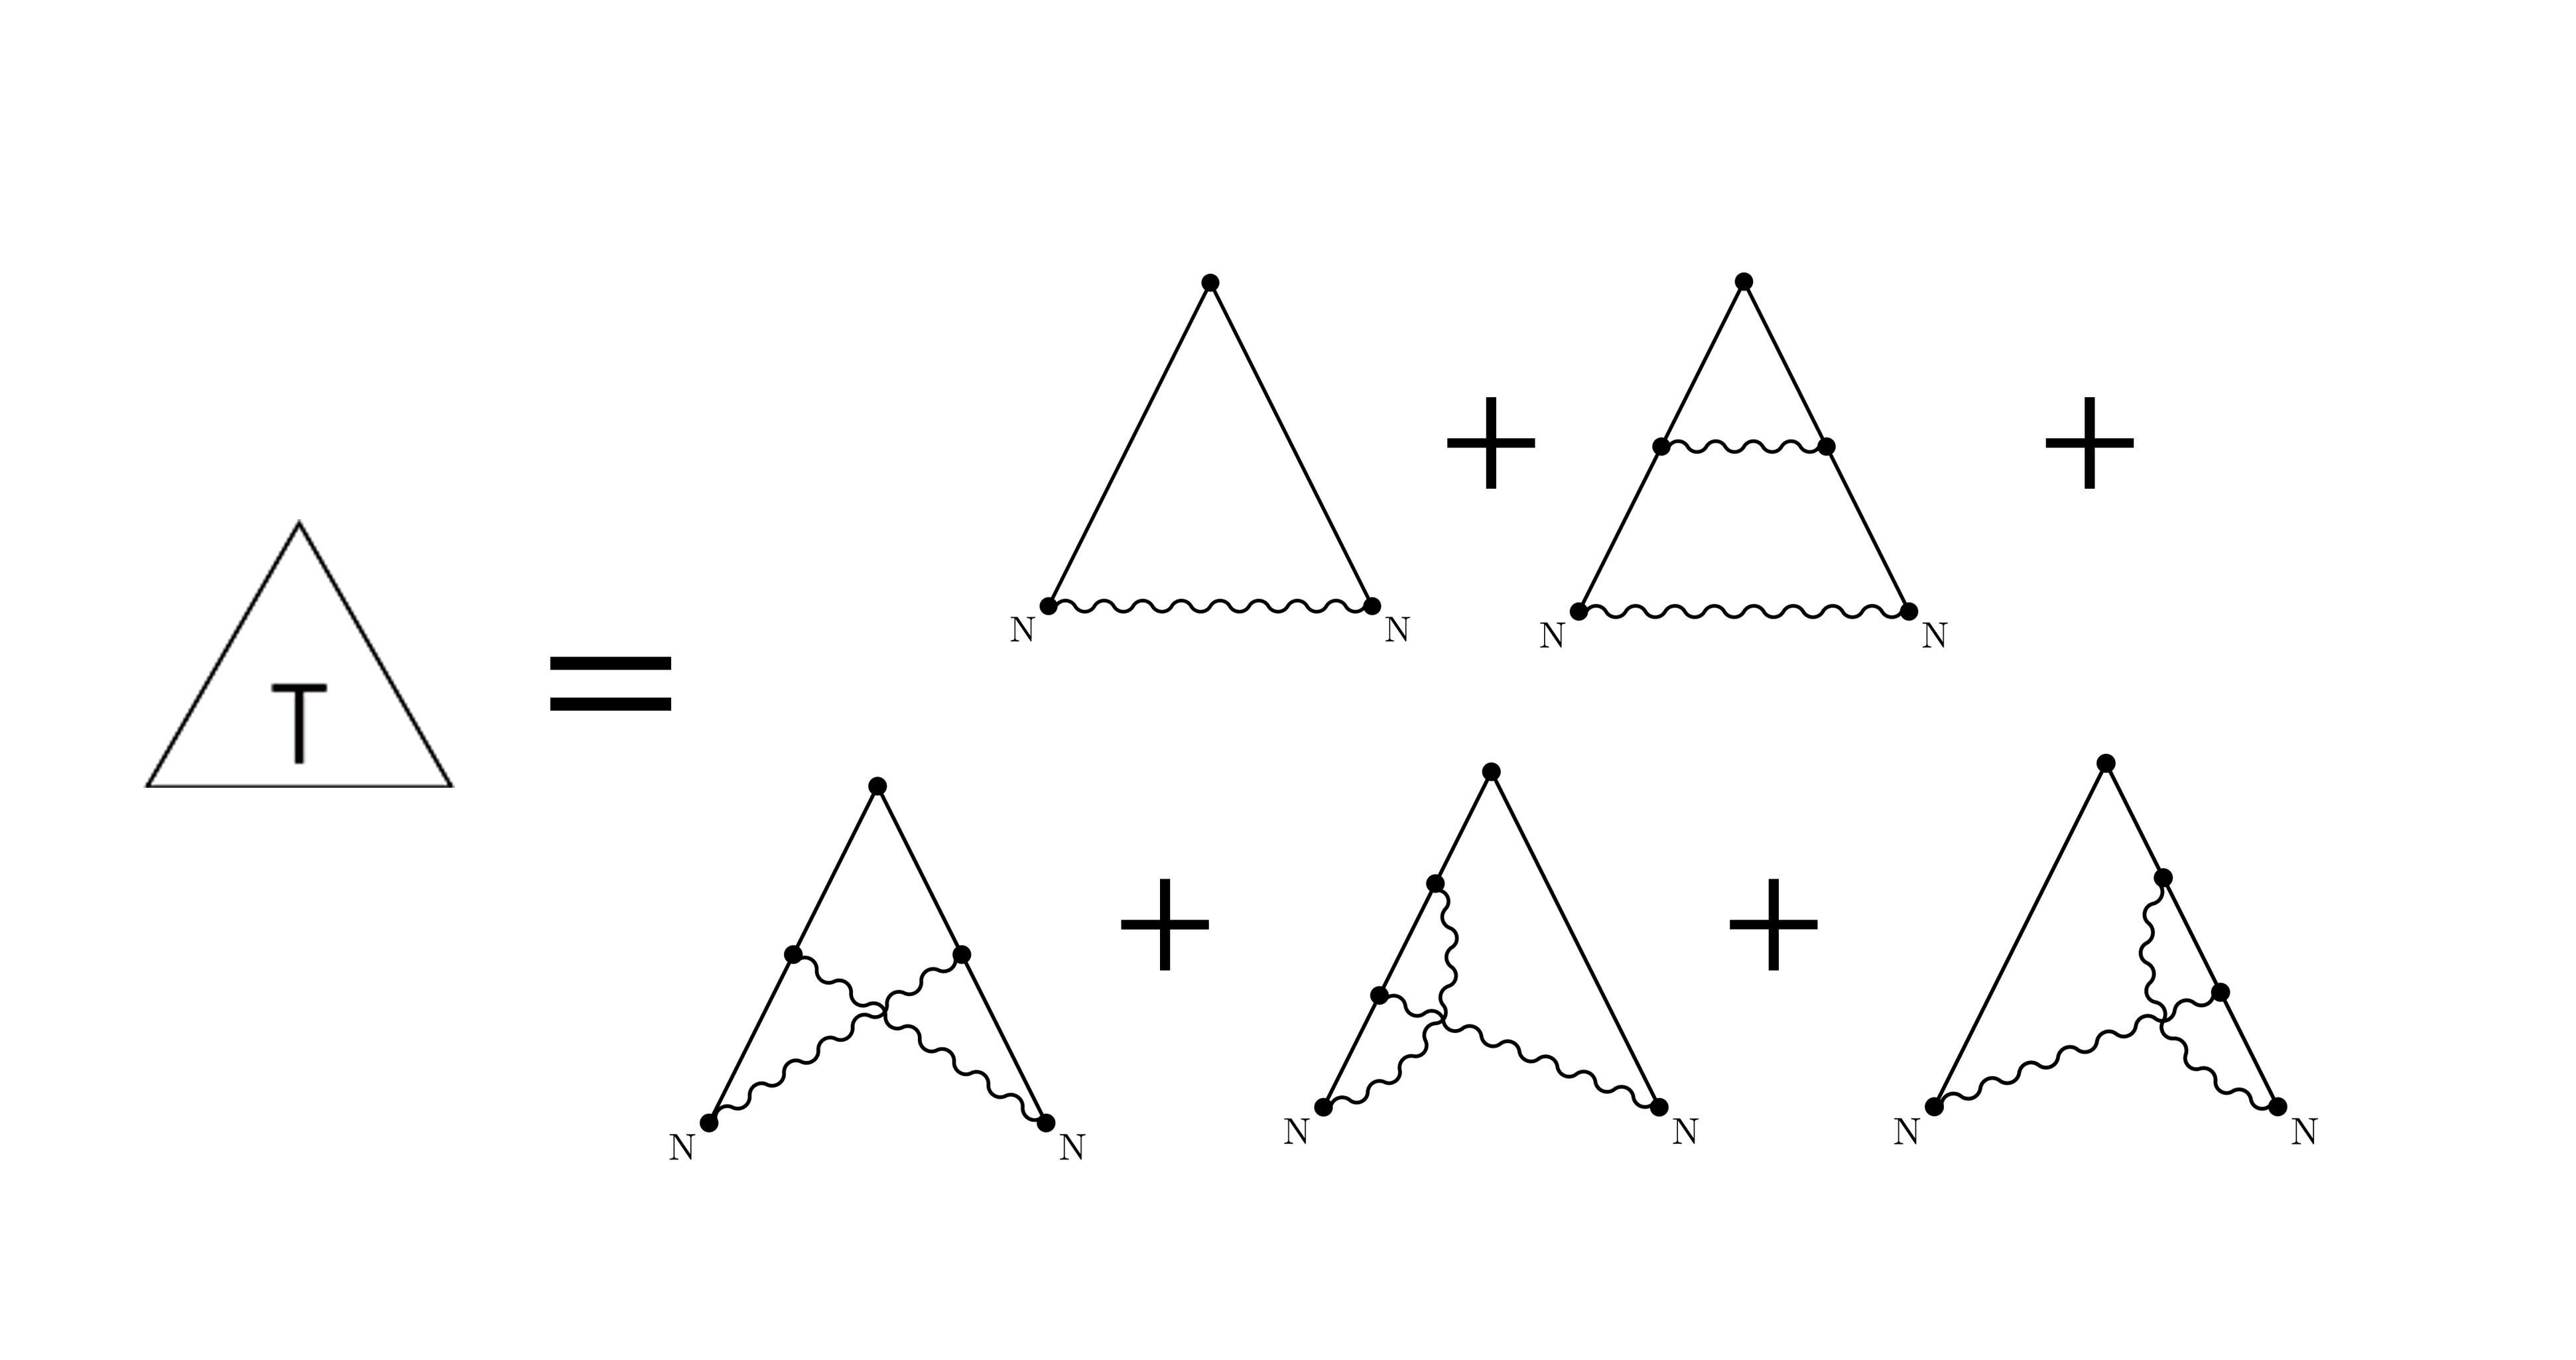
\includegraphics[width=12cm]{TexFigure/TOA_tmat.png}}
  \caption{Self-energy diagram for Five order expansion (TOA). The structure of T matrix was adopted.}
\end{figure}
\subsubsection*{Evaluation of correlation function}
The Correlation function for green’s function is defined as follows:
\begin{flalign}
  \begin{split}
\chi_{sp}(\tau)=\frac{1}{Z}\text{Tr}[e^{-S}P(\tau)P(0)] \\
=\text{Tr}[\mathcal{G}(\beta-\tau)P\mathcal{G}(\tau)P] + \text{Tr}[\tilde{T}(\beta,\tau)P]
  \end{split}
\end{flalign}
where $S$ is a action of system. The notation $\tilde{T}$ indicates:
\begin{flalign}
  \begin{split}
\tilde{T}(n,m) = \Delta\tau^2 \sum^n_{l=m}\bar{\mathcal{W}}^{(n-m)}_{l-m}\sum^m_{r=0}\bar{\mathcal{W}}^{(m)}_r\big[\mathcal{G}(n-l)T(l-r,m-r)\mathcal{G}(r)]
\end{split}
\end{flalign}
The indices of equations are related to how time has been ordered during the calculation.
There were new topological structure T has been applied. In the lowest expansion order, its structure is:
\begin{flalign}
  \begin{split}
T(\tau,\tau') = \big[P\mathcal{G}(\tau-\tau')P\mathcal{G}(\tau')P]\bar{\mathcal{W}}(\tau)
\end{split}
\end{flalign}
Which corresponding topological diagram is:
\begin{figure}[hbtp]
  \centerline{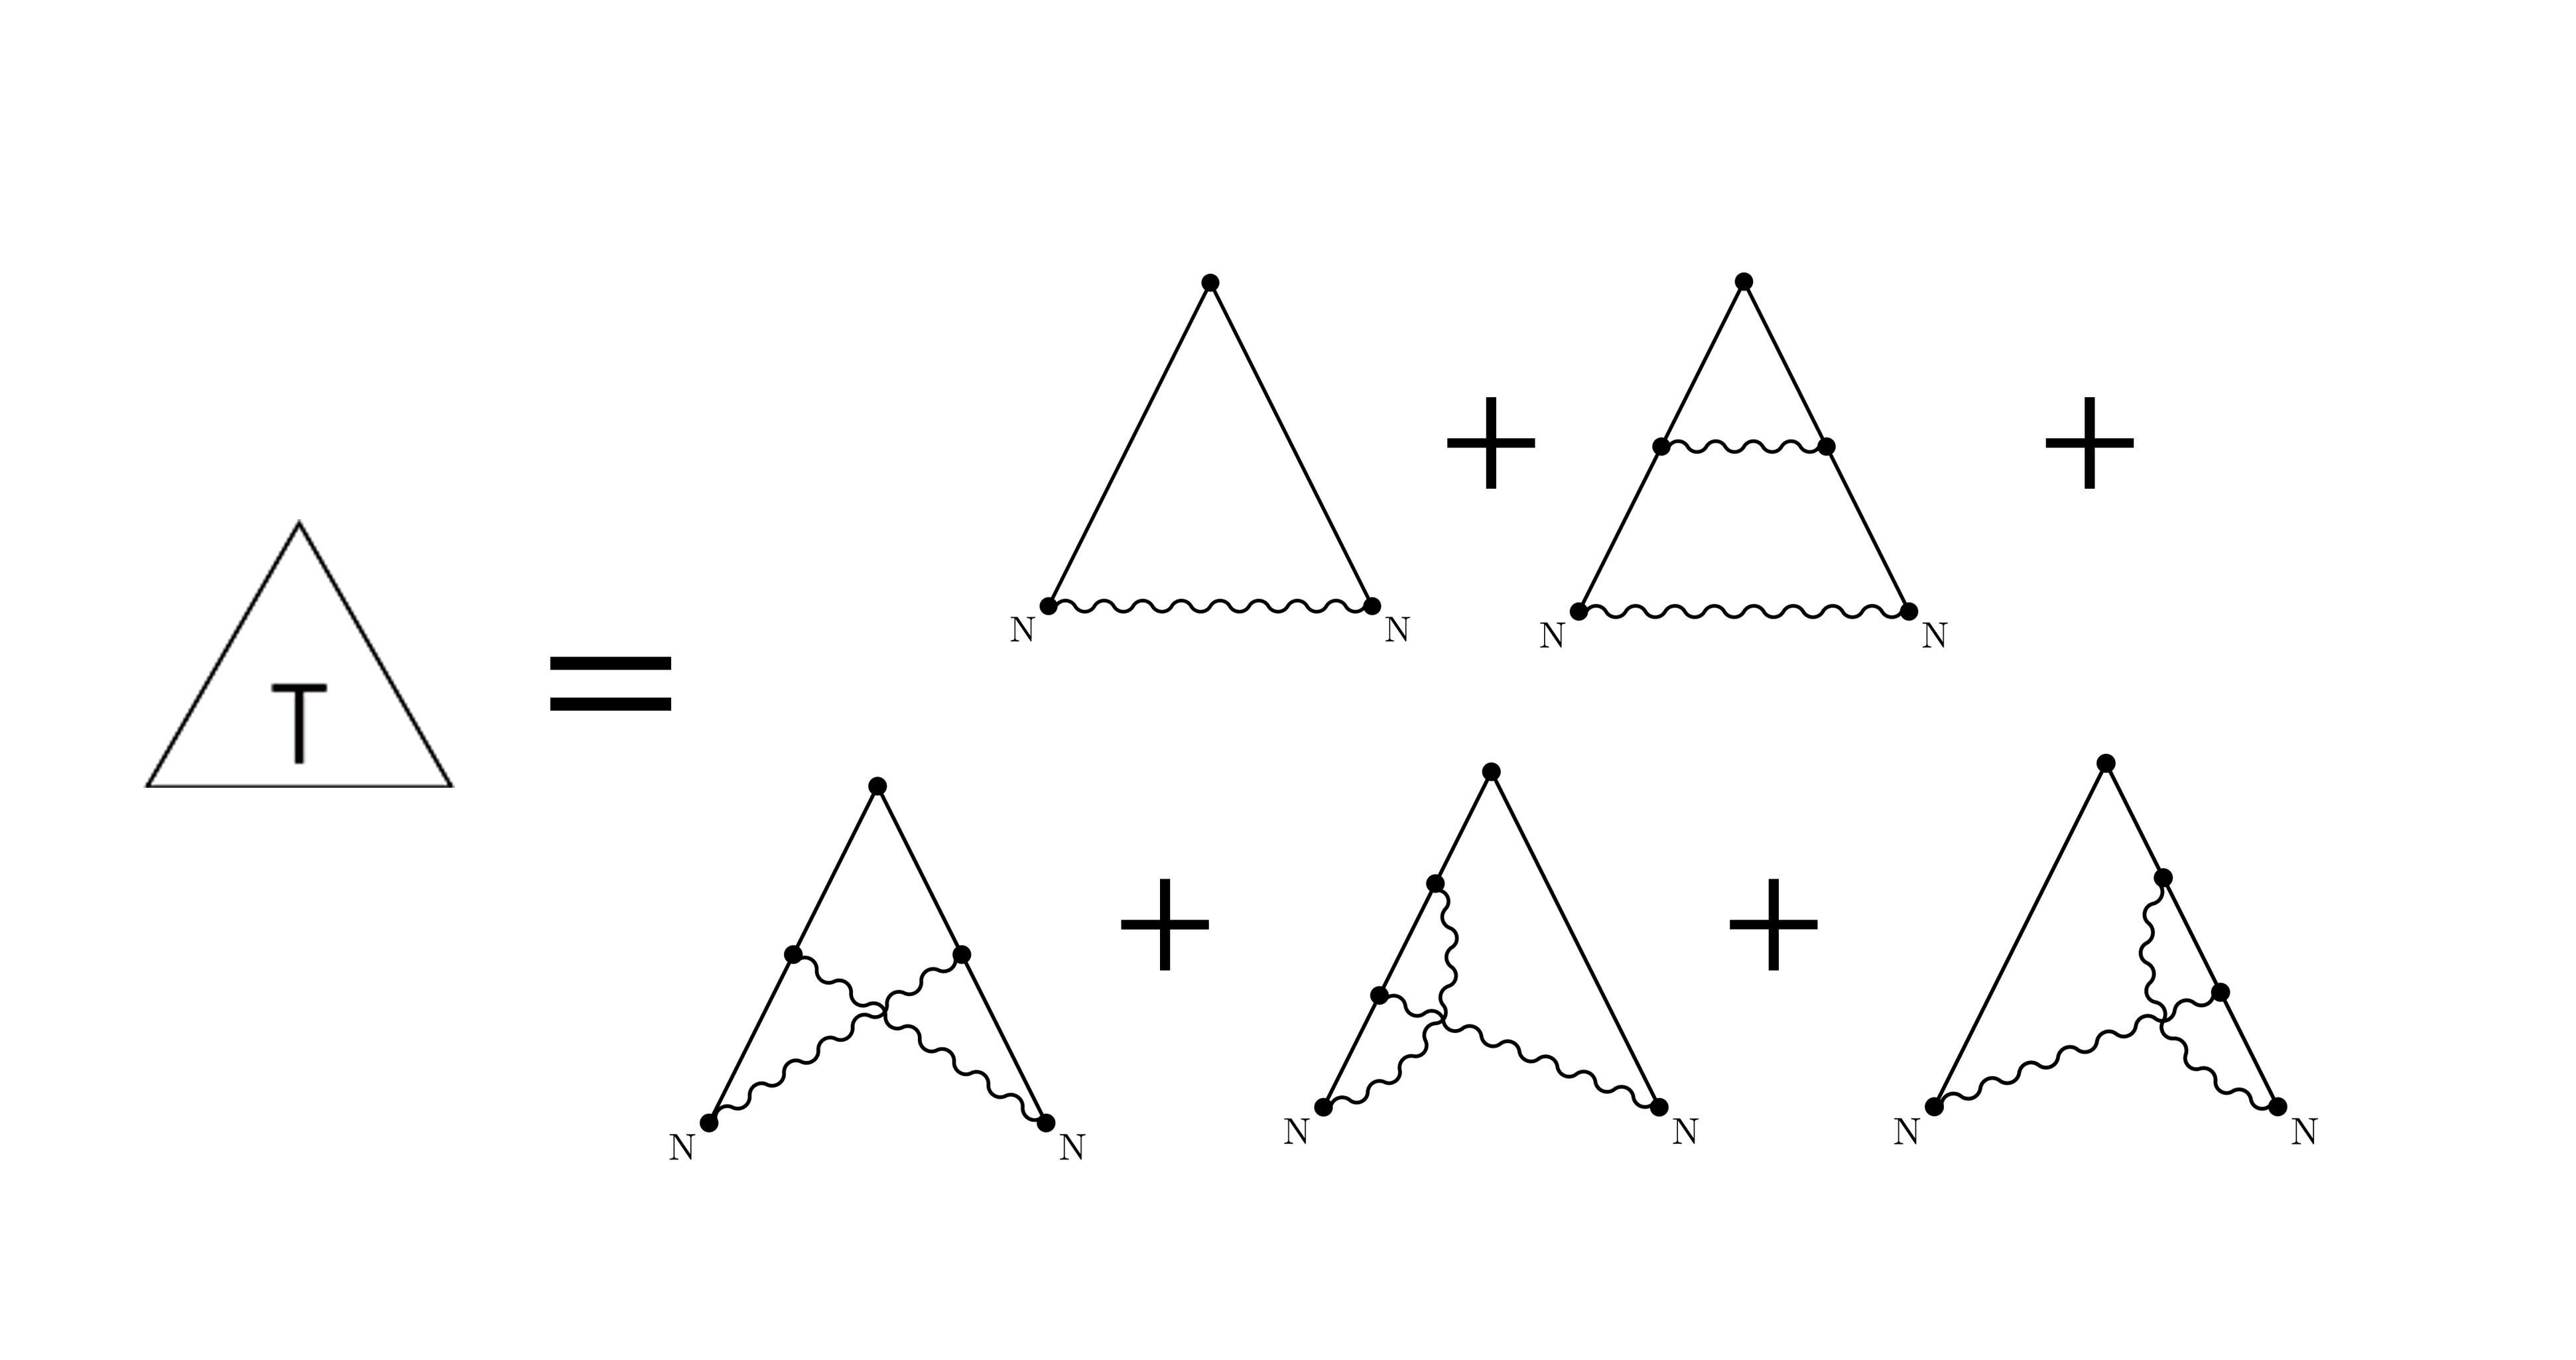
\includegraphics[width=5cm]{TexFigure/TOA_tmat.png}}
  \centerline{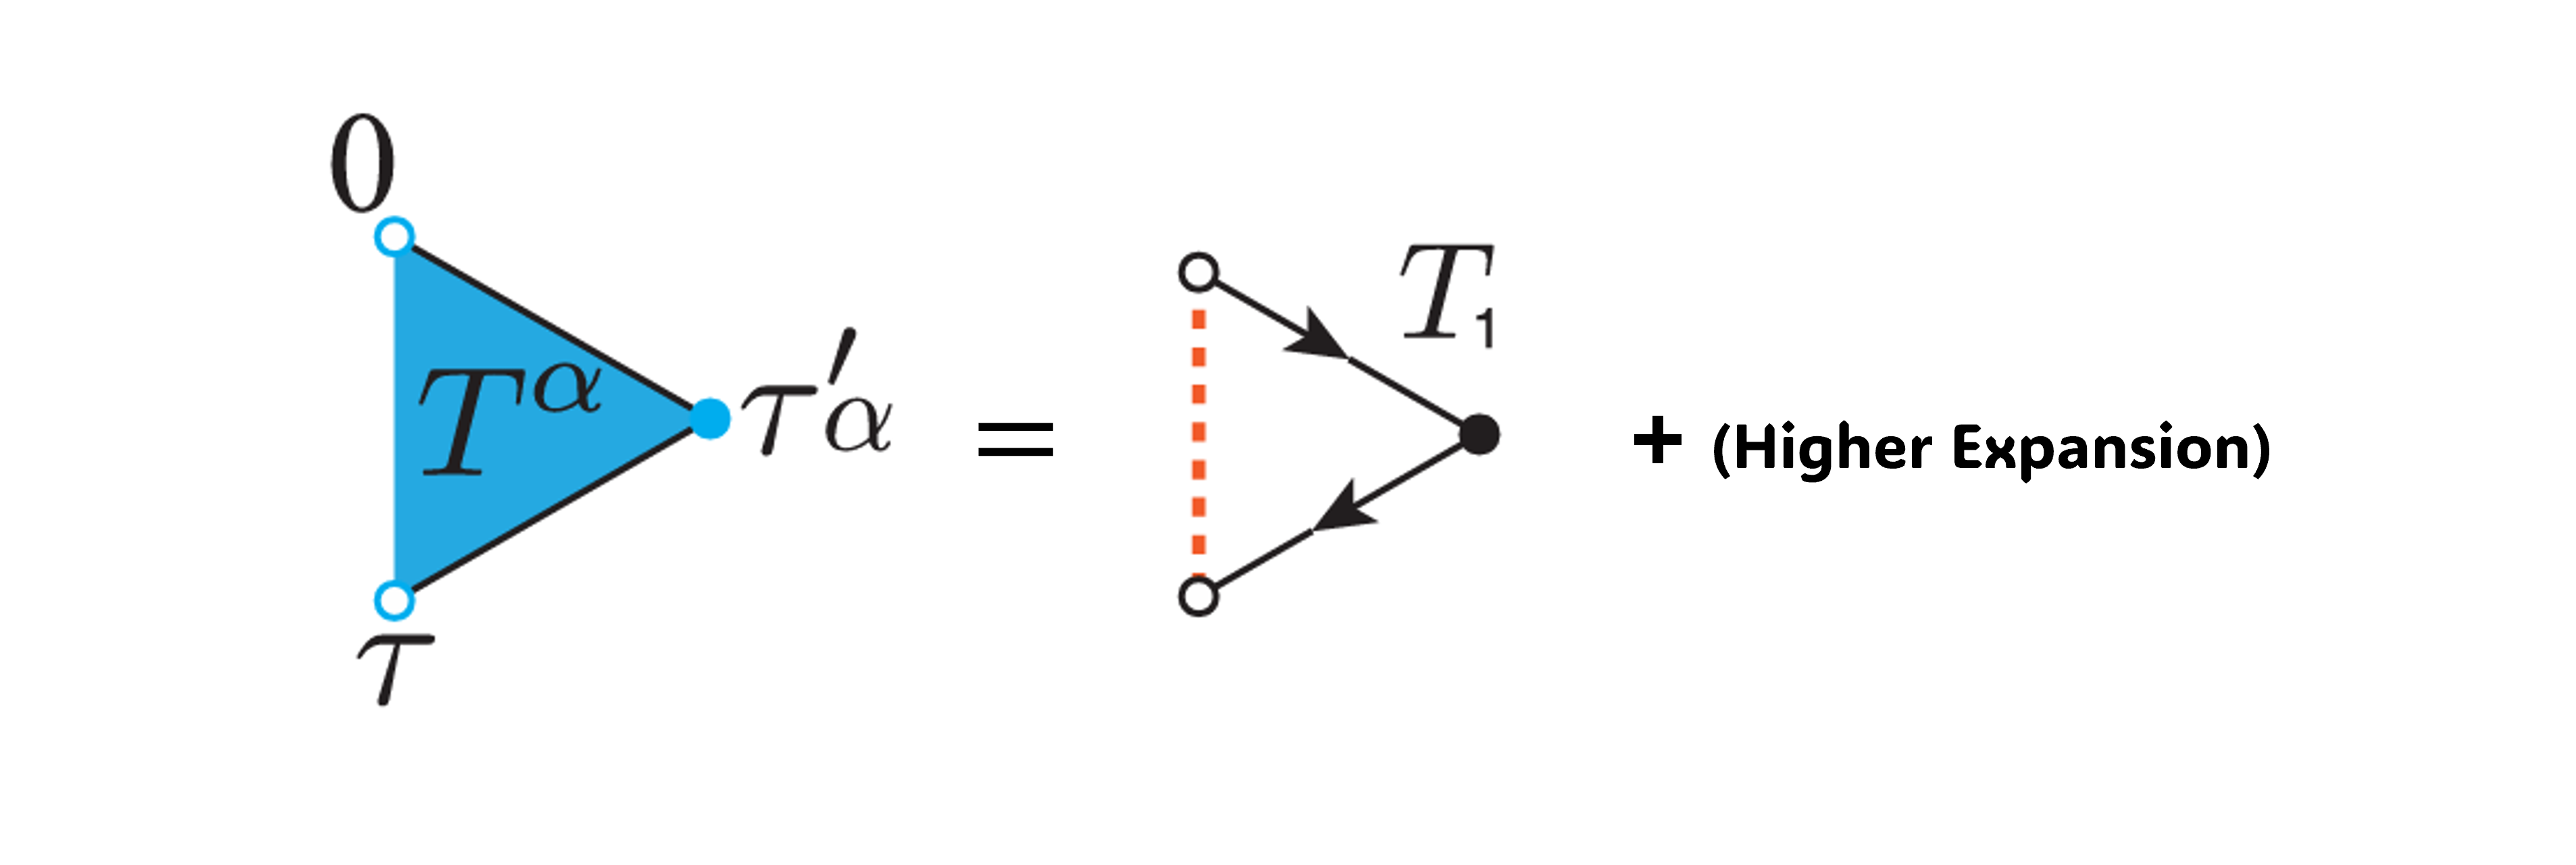
\includegraphics[width=12cm]{TexFigure/Tmat_diagram.png}}
  \centerline{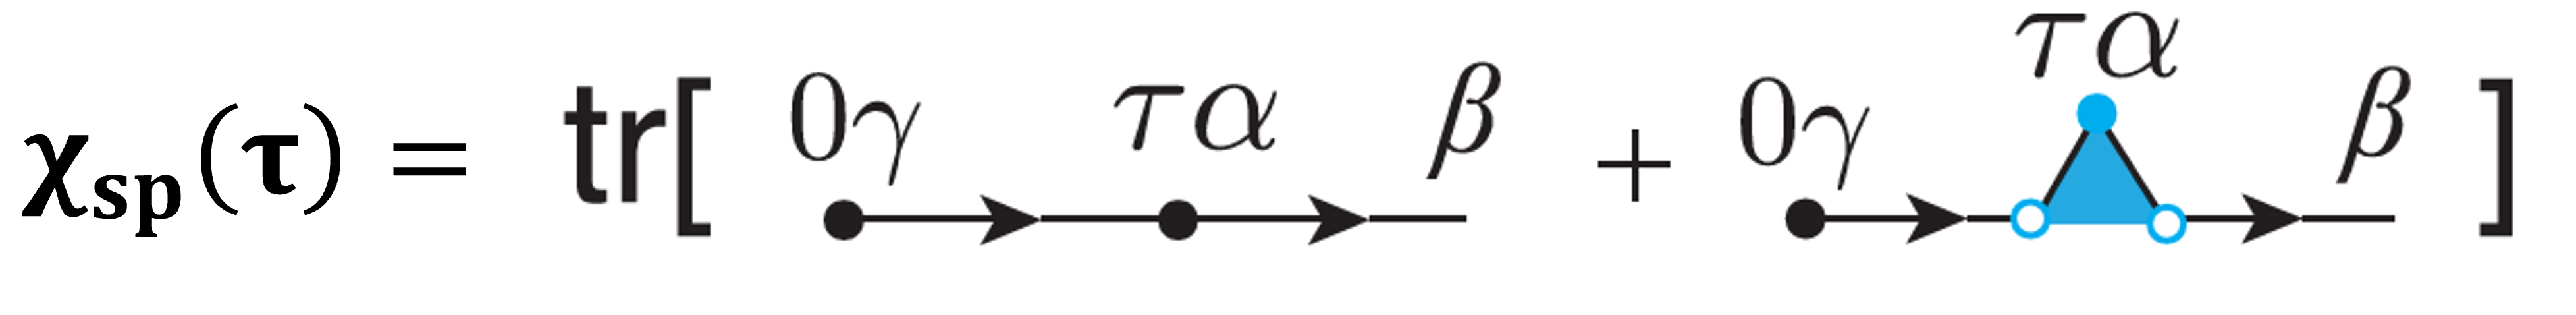
\includegraphics[width=12cm]{TexFigure/Chi_with_Tmat.png}}
  \caption{Specific diagram for T matrix\cite{PhysRevB.106.085124}}
\end{figure}
\end{spacing}
\pagebreak


\subsection{Applying to circuit hamiltonian model}
\begin{spacing}{1.5}
In our study, we consider that the total system turns out to be a thermal equilibrium state thus methodology using Matsubara’s method is available. To begin, we assume that each operator from RSJJ Hamiltonian mapped toward the general impurity model:
\begin{table}[htbp]
  \centering
  \renewcommand{\arraystretch}{1.2}
  \begin{tabular}{@{}ccc@{}}
  \toprule
  \textbf{Hamiltonian} &\textbf{RSJJ} & \textbf{Impurity} \\ 
  \midrule
  $H_{\text{bath}}$ &   $\sum_k \hbar\omega_k\hat{b}_k^\dagger\hat{b}_k$ & $\sum_n\epsilon_n\hat{b}_n^\dagger\hat{b}_n$ \\
  $H_\text{int}$ & $\sum_k g_k \hat{N}(\hat{b}^\dagger_k + \hat{b_k})$ & $\sum_{m,n} [V_{m,n}(t) c_m^\dagger b_n + \text{H.c.}]$ 
\end{tabular}
\caption{Comparison with term from Circuit hamiltonian and impurity solver}
\end{table}
More specifically, each parameter has corresponding relations,
\begin{flalign}
  \begin{split}
\hbar\omega_k &\rightarrow \epsilon_n \\
g_k &\rightarrow V_{m,n}\\ 
\hat{N} &\rightarrow \hat{c}^\dagger_m (\hat{c}_m) \\ 
\hat{b}_k^\dagger (\hat{b}_k) &\rightarrow \hat{b}_n^\dagger (\hat{b}_n)
\end{split}
\end{flalign}
Using the relations, we can calculate the system’s partition function as we dealt with in the eqn(2.44). 
\subsubsection*{Calculation of bosonic action}
To focus our attention on the local system where we are interested, we calculate the expectation value of partition function in the aspects of the bath, which eliminates the effects of the bath by evaluating the system dynamics in bath points of view:
\begin{flalign}
  \begin{split}
Z &= Z_{\text{bath}}\text{Tr}_{JJ}\bigg[\frac{\text{Tr}[e^{-\beta H_\text{bath}}U_{sys}(\tau)]}{\text{Tr}[e^{-\beta H_\text{bath}}]}\bigg] \\ 
&= Z_\text{bath}\text{Tr}_{\text{JJ}}[\langle \mathcal{T}_\tau e^{-\int^\beta_0 H_\text{loc}(\tau) + H_\text{bath} + H_\text{int}}\rangle_\text{b}]
\end{split}
\end{flalign}
Here the term $\text{JJ}$ means tracing out the effect of local system, in our case, Josephson junction system, and term is tracing out the effect of bosonic effect, which is $\bra{n_b}\mathcal{O}\ket{n_b}$, $n_b$ is number operator for bosonic field operator, $\mathcal{O}$ is physical quantity to calculate.
To expand the interaction term, we can rewrite the equation into :
\begin{flalign}
  \begin{split}
Z=Z_{\text{bath}}\text{Tr}_{JJ}[\langle \mathcal{T}_\tau e^{-\int^\beta_0 H_\text{loc}(\tau) + H_\text{bath}}\sum_l Z_l\rangle_\text{b}]
\end{split}
\end{flalign}
Here, $l$ corresponds with the number of highest order of perturbative expansion. The derivation of Term $Z_k$ begins from
\begin{flalign}
  \begin{split}
 \mathcal{T}_\tau e^{-\int^\beta_0 H_{\text{int}}(\tau)} \approx 1 -\int^{\beta}_0 H_{\text{int}}(\tau) d\tau +\frac{1}{2} \int^\beta_0 H_{\text{int}}(\tau_1)H_{\text{int}}(\tau_2)d\tau_1 d\tau_2 + \cdots
\end{split}
\end{flalign}
And 
\begin{flalign}
  \begin{split}
Z_l =&\sum_{k_1 \cdots k_l}\sum_{k'_1 \cdots k'_l} g_{k_1}g_{k'_1}g_{k_2}g_{k'_2} \cdots g_{k_l}g_{k'_l} \int^\beta_0 d\tau_1 \int^\beta_{\tau_1}d\tau_2 \cdots\int^\beta_{\tau_{{l-1}}}d\tau_{l} \int^\beta_0 d\tau_1 \int^\beta_{\tau'_1}d\tau'_2 \cdots\int^\beta_{\tau'_{{l-1}}}d\tau'_{l} 
\\ & \times \hat{N}(\tau_1)\hat{b}^\dagger_{k_1}(\tau_1)\hat{N}(\tau'_1)\hat{b}_{k'_1}(\tau'_1)  \hat{N}(\tau_2)\hat{b}^\dagger_{k_2}(\tau_2)\hat{N}(\tau'_2)\hat{b}_{k'_2}(\tau'_2) \cdots \hat{N}(\tau_{l})\hat{b}^\dagger_{k_l}(\tau_{l})\hat{N}(\tau'_{l})\hat{b}_{k'_l}(\tau'_{l})
\end{split}
\end{flalign}
Here the lower index $k_i$ indicates the oscillation mode of the ith harmonic oscillator from bath that is represented as a pair of bosonic creation and annihilation operators. The number $\frac{1}{k_l !}$ was eliminated due to considering all permutations during ordering time.
Notice that, \textit{1.} $k_i =k'_j$ \textit{ for all }(i,j)  , 
\textit{2. } $\hat{N}$ \textit{ and  } $\hat{b}_k^\dagger(\hat{b_k})$\textit{  are defined on different vector space , thus   }
$[\hat{N},\hat{b}^\dagger (\hat{b})] = 0$ , we can adjust $Z_l$ as follows :
\begin{flalign}
  \begin{split}
Z_l = &\sum_{k_1 \cdots k_l} (g_{k_1}g_{k_2} \cdots g_{k_l})^2\int^\beta_0 d\tau_1 \int^\beta_{\tau_1}d\tau_2 \cdots\int^\beta_{\tau_{k_{l-1}}}d\tau_{k_l} \int^\beta_0 d\tau_1 \int^\beta_{\tau'_1}d\tau'_2 \cdots\int^\beta_{\tau'_{k_{l-1}}}d\tau_{k_l} \\ 
&\times \hat{N}(\tau_1)\hat{b}^\dagger_{k_1}(\tau_1)\hat{b}_{k_1}(\tau'_1)\hat{N}(\tau'_1)  \hat{N}(\tau_2)\hat{b}^\dagger_{k_2}(\tau_2)\hat{b}_{k_2}(\tau'_2)\hat{N}(\tau'_2) 
\cdots \hat{N}(\tau_{k_l})\hat{b}^\dagger_{k_l}(\tau_{k_l})\hat{b}_{k_l}(\tau'_{k_l})\hat{N}(\tau'_{k_l})
\end{split}
\end{flalign}
To calculate the effect of bath, the form of the equation turns out:  
\begin{flalign}
  \begin{split}
\langle & \mathcal{T}_\tau e^{-\int^\beta_0 H_\text{loc}(\tau) + H_\text{bath}}\sum_l Z_l\rangle_\text{b} \\ 
&= \mathcal{T}_\tau e^{-\int^\beta_0 H_{loc}}\langle \mathcal{T}_\tau e^{-\int^\beta_0  H_\text{bath}}\sum_l Z_l\rangle_\text{b} \\ 
&=\mathcal{T}_\tau e^{-\int^\beta_0 H_{loc}}\langle \mathcal{T}_\tau e^{-\int^\beta_0  H_\text{bath}}\sum_l \text{(bosonic terms)}\rangle_\text{b} \\ 
\times \int^\beta_0 d\tau_1 \int^\beta_{\tau_1}d\tau_2 \cdots\int^\beta_{\tau_{k_{l-1}}} & d\tau_{k_l} \int^\beta_0 d\tau_1 \int^\beta_{\tau'_1}d\tau'_2 \cdots\int^\beta_{\tau'_{k_{l-1}}}d\tau_{k_l}
 \hat{N}(\tau_1)\hat{N}(\tau'_1)  \hat{N}(\tau_2)\hat{N}(\tau'_2) 
\cdots \hat{N}(\tau_{k_l})\hat{N}(\tau'_{k_l})
\end{split}
\end{flalign}
Here, each bosonic term contains a calculation of form $\langle \hat{b}^\dagger_{k_1}(\tau_1)\hat{b}_{k_1}(\tau'_1)\hat{b}^\dagger_{k_2}(\tau_2)\hat{b}_{k_2}(\tau'_2)\cdots\hat{b}^\dagger_{k_l}(\tau_l)\hat{b}_{k_l}(\tau'_l)\rangle_\text{b}$, where Wick’s theorem is available. 
Before applying Wick’s theorem to a given equation, notice that there are natural restrictions due to the independence of harmonic oscillators in the bath which do not interact with each others, leading to only one available property for contraction,
\begin{flalign}
  \begin{split}
\langle \hat{b}^\dagger_{k_1}(\tau_1)\hat{b}_{k_1}(\tau'_1)\hat{b}^\dagger_{k_2}(\tau_2)\hat{b}_{k_2}(\tau'_2)&\cdots\hat{b}^\dagger_{k_l}(\tau_l)\hat{b}_{k_l} (\tau'_l)\rangle_\text{b} \\
 = &\langle \hat{b}^\dagger_{k_1}(\tau_1)\hat{b}_{k_1}(\tau'_1)\rangle_\text{b} \langle\hat{b}^\dagger_{k_2}(\tau_2)\hat{b}_{k_2}(\tau'_2)\rangle_\text{b}\cdots\langle\hat{b}^\dagger_{k_l}(\tau_l)\hat{b}_{k_l} (\tau'_l)\rangle_\text{b} 
 \\ & +\langle \hat{b}_{k_1}(\tau'_1)\hat{b}^\dagger_{k_1}(\tau_1)\rangle_\text{b} \langle\hat{b}_{k_2}(\tau'_2)\hat{b}^\dagger_{k_2}(\tau_2)\rangle_\text{b}\cdots\langle\hat{b}_{k_l}(\tau'_l)\hat{b}^\dagger_{k_l} (\tau_l)\rangle_\text{b}
\end{split}
\end{flalign}
Which is full bosonic term turn out to sum of multiplication of single bosonic Green’s function.
It is known that when the ensemble Hamiltonian, aimed at observing a certain physical quantity, takes the form of a harmonic oscillator, 
it can be expressed as $\hat{a}^\dagger(\tau) = e^{E\tau} , \hat{a}(\tau) = e^{-E\tau}\hat{a}$  where $E$ is a eigenvalue of Hamiltonian. 
Using this formula, each single Green’s function can be calculated as:
\begin{flalign}
  \begin{split}
\langle e^{-\omega_k \tau}\hat{b}^\dagger_k e^{-\omega_k \tau'}\hat{b}_k\rangle_\text{b} &= \langle e^{\omega_p (\tau-\tau')}\hat{b}^\dagger_k\hat{b}_k\rangle_\text{b} = e^{\omega_k \tau}n_\text{B}(\omega_k) \qquad (\tau>\tau') \\
\langle e^{-\omega_k \tau}\hat{b}_k e^{-\omega_k \tau'}\hat{b}^\dagger_k\rangle_\text{b} = \langle e^{\omega_p (\tau-\tau')}\hat{b}_k\hat{b}^\dagger_k\rangle_\text{b} &= \langle e^{\omega_p (\tau-\tau')}(1+\hat{b}_k^\dagger\hat{b}_k\rangle_\text{b} = e^{\omega_k (\tau-\tau')}(1+n_\text{B}(\omega_k)) \qquad (\tau<\tau')
  \end{split}
\end{flalign}
By multiplying the corresponding coupling parameter $g_k^2$ in mode $k$ , the full equation becomes :
\begin{flalign}
  \begin{split}
\langle \mathcal{T}_\tau e^{-\int^\beta_0  H_\text{bath}} Z_l\rangle_\text{b} =g^2_{k_1}\big(e^{\omega_{k_1}(\tau_1-\tau'_1)}(\theta(\tau_1-\tau'_1)n_\text{B}(\omega_{k_1})+\theta(\tau'_1-\tau_1)[1+n_\text{B}(\omega_{k_1})])\big) \\
\times g^2_{k_2}\big(e^{\omega_{k_2}(\tau_2-\tau'_2)}(\theta(\tau_2-\tau'_2)n_\text{B}(\omega_{k_2})+\theta(\tau'_2-\tau_2)[1+n_\text{B}(\omega_{k_2})])\big)\\
\vdots\\
\times g^2_{k_l}\big(e^{\omega_{k_l}(\tau_l-\tau'_l)}(\theta(\tau_l-\tau'_l)n_\text{B}(\omega_{k_l})+\theta(\tau'_l-\tau_l)[1+n_\text{B}(\omega_{k_l}]))\big)
\end{split}
\end{flalign}
In the general approach, the term that corresponds to $\mathcal{W}$  from pseudo-particle solver can be expressed as follows:
\begin{flalign}
  \begin{split}
\mathcal{W}(\tau)=\begin{cases}  \sum_k |g_k|^2 e^{\omega_k \tau}n_{\text{B}}(\omega_k) \qquad (\tau>0) \\ \sum_k |g_k|^2 e^{\omega_k \tau}[1+n_{\text{B}}](\omega_k) \quad (\tau<0) \end{cases}
  \end{split}
\end{flalign}
And instead of notation $\mathcal{\bar{W}}$, we use $V_k(\tau)$  to representing simultaneously for retarded and advanced cases, 
\begin{flalign}
  \begin{split}
V_k(\tau) = e^{-\omega_k\tau}\theta(-\tau)n_B(\omega_k \beta)  + e^{\omega_k\tau}\theta(\tau)(1+n_B(\omega_k \beta))
\end{split}
\end{flalign}
In which we can rewrite as the form of:
\begin{flalign}
  \begin{split}
V_k(\tau)= e^{-\omega_k\tau} \frac{\cosh{\frac{\omega_k}{2}}}{\sinh{\frac{\omega_k}{2}}}
\end{split}
\end{flalign}

\end{spacing}
\end{document}